% Provenance (never printed): see sources/outline_sources.md (Year 3: elastic waves
% recalled from the physics books; rays in a spherical Earth; travel-time tables;
% surface waves and dispersion; normal modes, told; linear inverse problems and
% seismic tomography). Brief: sources/book5/BRIEFS.md, ch. 1. Curves from
% figdata/bachelor-3/ray_tracing.py, love_dispersion.py, tomo_checkerboard.py;
% exercise and problem values in the Book 5 scratch calculator calc/ch01.py.
\chapter{भूकंप विज्ञान और पृथ्वी का प्रतिचित्रण}\label{ch:b3:seismology-imaging}\setlength{\emergencystretch}{3em}

22 मई 1960 को, सार्वभौमिक समय 19:11 बजे, 1900 के बाद से दर्ज सबसे बड़े
भूकंप ने दक्षिणी चिली के तट पर क्षेपण क्षेत्र को तोड़ा, जिसका परिमाण 9.5 था।
% ledger: usgs5:chile1960
इसकी P तरंगें ग्रह के दूसरी ओर के स्टेशनों तक लगभग बीस मिनट
बाद पहुँचीं; इसकी पृष्ठ-तरंगें पृथ्वी का कई बार चक्कर लगा गईं; और कई दिनों के
बाद तक सबसे धीमे उपकरणों ने पूरी पृथ्वी को कंपन करते हुए दर्ज किया,
जिसके आवर्तकाल एक घंटे के निकट थे, मानो कोई ठोकी गई घंटी हो। इनमें से प्रत्येक संकेत
अपने पार की गई चट्टानों के बारे में जानकारी लिए चलता है। लाखों
ऐसी तरंगों के आगमन-कालों से, जिन्हें हज़ारों केंद्रों पर पढ़ा गया, भूकंपविज्ञानियों ने न केवल
नीचे याद किया गया स्तरित पृथ्वी मॉडल, बल्कि
प्रावार के त्रि-आयामी प्रतिचित्र भी बनाए हैं, जिनमें डूबती स्लैब और उठते प्लूम
उन क्षेत्रों के रूप में दिखते हैं जहाँ तरंगें औसत से कुछ तेज़ या धीमी चलती हैं। यह अध्याय बताता है कि:
किरणें गोलीय पृथ्वी में कैसे चलती हैं, पृष्ठ-तरंगें भूपर्पटी
और प्रावार को उनके परिक्षेपण से कैसे खँगालती हैं, और पूरे
ग्रह के मुक्त दोलनों का वर्णन कैसे होता है, और कुछ हज़ार यात्रा-काल किस प्रकार
एक रैखिक \omterm{def:b3:seismology-imaging:inverse}{प्रतिलोम समस्या} हल करके एक चित्र में बदले जाते हैं।

\begin{recall}
समदैशिक प्रत्यास्थ ठोस में दो प्रकार की काय-तरंगें चलती हैं: P तरंगें, जिनकी
चाल $\alpha = \sqrt{(K + \tfrac43\mu)/\rho}$ है, और S तरंगें, जिनकी
चाल $\beta = \sqrt{\mu/\rho}$ है, जहाँ $K$ और $\mu$ क्रमशः थोक और अपरूपण मापांक हैं,
और $\rho$ घनत्व है; S तरंगें द्रव से होकर नहीं गुज़रतीं (भौतिकी की पुस्तकों के स्नातक वर्ष 3 खंड,
सतत प्रत्यास्थता वाले अध्याय में)। जिस तरंग का कला-वेग
अपनी आवृत्ति पर निर्भर करता है, वह परिक्षेपी है; उसकी ऊर्जा समूह
वेग $U = \mathrm d\omega/\mathrm dk$ से चलती है (भौतिकी की पुस्तकों के स्नातक वर्ष 2 खंड में,
तरंगों वाले अध्याय में)। एक परिबद्ध प्रत्यास्थ पिंड असतत
प्रसामान्य विधाओं में मुक्त रूप से कंपन करता है (उसी खंड में)। किसी केंद्र की अधिकेंद्री दूरी $\Delta$ वह कोण है
पृथ्वी के केंद्र पर अधिकेंद्र और केंद्र के बीच बनता है; यात्रा-काल वक्र
वक्र $\Delta$ के विरुद्ध पहले आगमन का समय देता है, और क्रोड प्रत्यक्ष P तरंगों के लिए
एक छाया क्षेत्र बनाता है (पुस्तक 2, कक्षा 11)। संदर्भ पृथ्वी मॉडल,
भूकंपीय असांतत्य और हेड तरंग पुस्तक 3 (स्नातक वर्ष 1) में देखे गए थे,
उसके स्तरित पृथ्वी वाले अध्याय में। न्यूनतम वर्ग और गाउसीय
त्रुटि-नियम गणित की पुस्तकों के हैं।
\end{recall}

\section{गोलीय पृथ्वी में किरणें}

भूकंपीय तरंगाग्र, अपने स्रोत से दूर और ऐसे माध्यम में जिसके गुण
तरंगदैर्घ्य भर में धीरे बदलते हैं, उसकी किरणों द्वारा अनुसरित किए जा सकते हैं: ऐसे वक्र
जो हर जगह तरंगाग्र के लंबवत होते हैं और जिनके अनुदिश ऊर्जा चलती है।
एकसमान चाल वाले माध्यम में किरणें सीधी होती हैं; जहाँ चाल बदलती है वहाँ वे
स्नेल के अपवर्तन नियम से मुड़ती हैं। पृथ्वी में चालें मुख्यतः
गहराई पर निर्भर करती हैं, इसलिए पहला मॉडल गोलीय सममित लिया जाता है: विचाराधीन तरंग की
(P या S) चाल $v(r)$ केवल त्रिज्या $r$ का फलन होती है।

\begin{theorem}[गोलीय पृथ्वी में स्नेल का नियम]\label{thm:b3:seismology-imaging:snell}
तरंग-चाल $v(r)$ वाली गोलीय सममित पृथ्वी में मान लीजिए $i$ वह कोण है
जो किरण और त्रिज्या $r$ वाले बिंदु पर उस त्रिज्या के बीच बनता है। पूरी किरण के अनुदिश,
\[
  \frac{r\sin i}{v(r)} = p
\]
स्थिर रहता है।
\end{theorem}

\begin{proof}
पृथ्वी को पतले संकेंद्रीय कोशों से बदला जाता है, जिनमें से हर एक में चाल एकसमान होती है। किसी
कोश के भीतर किरण एक सरल रेखा होती है; केंद्र से दूरी $d$ पर स्थित एक सरल रेखा
त्रिज्या $r$ के गोले को कोण $i$ पर इस प्रकार काटती है कि
$r\sin i = d$ होता है (केंद्र, लंब के पाद और बिंदु से बना समकोण
त्रिभुज), इसलिए $r\sin i$ कोश के ऊपरी और निचले सिरे पर एक समान होता है। तो
त्रिज्या $r$ की उस सीमा पर जो दो कोशों के बीच है, जिनकी
चालें $v_1$ और $v_2$ हैं, स्नेल का नियम देता है $\sin i_1/v_1 = \sin i_2/v_2$, इसलिए
$r\sin i/v$ उसके आर-पार सतत है। कोश के भीतर $v$ स्थिर है और
$r\sin i$ स्थिर है, इसलिए वहाँ $r\sin i/v$ भी स्थिर है। अतः
पूरी किरण के अनुदिश स्थिर है; कोशों की मोटाई को
शून्य की ओर जाने देने पर सतत $v(r)$ के लिए परिणाम मिलता है।
\end{proof}

\begin{definition}[किरण प्राचल, पलटाव बिंदु]\label{def:b3:seismology-imaging:ray-parameter}
गोलीय सममित पृथ्वी में किसी किरण का स्थिरांक $p = r\sin i/v(r)$
उसका \emph{किरण प्राचल}\index{किरण प्राचल} है, जिसकी इकाई सेकंड प्रति रेडियन है।
पृष्ठ पर यह $p = R\sin i_0/v_0$ है, जहाँ $i_0$ निर्गम-कोण है और $v_0$
पृष्ठ पर की चाल है। वह बिंदु जहाँ किरण क्षैतिज ($i = \ang{90}$) होती है,
वही उसका \emph{पलटाव बिंदु}\index{पलटाव बिंदु} है,
त्रिज्या $r_t$ पर, जहाँ
\[
  \frac{r_t}{v(r_t)} = p .
\]
इसके नीचे किरण फिर ऊपर उठती है, पलटाव बिंदु से गुज़रने वाली
त्रिज्या के सापेक्ष सममित होती है।
\end{definition}

मान लीजिए $\eta(r) = r/v(r)$। प्राचल $p$ वाली किरण केवल वहीं विद्यमान हो सकती है जहाँ
$\eta \ge p$, क्योंकि $\sin i = p/\eta \le 1$। यदि $\eta$ गहराई के साथ घटता है, जैसा कि
अधिकांश प्रावार में होता है, तो हर किरण उस गहराई पर पलटती है जहाँ $\eta$
$p$ तक गिर चुका होता है, और अधिक खड़ी निकलने वाली (छोटे $p$ वाली) किरणें अधिक गहराई पर पलटती हैं।
जहाँ $\eta$ गहराई के साथ \emph{बढ़ता} है, क्योंकि चाल गहराई के साथ तेज़ी से
घटती है (कोर–प्रावार सीमा पर ऐसा होता है, जहाँ P चाल 13.7 से
\qty{8.0}{km.s^{-1}} तक गिरती है), % ledger: ak135:cmb
कोई किरण नहीं पलट सकती: किरणें नीचे की ओर मुड़ती हैं, परत को पार करती हैं और दूर जाकर निकलती हैं।
ऐसी छलांग पृष्ठ पर एक छाया डालती है।

\begin{omfigure}
\begin{tikzpicture}[font=\small, x=1.6cm, y=1.6cm]
% concentric shells, centre O at (0,-9) (outside the picture); ray computed by
% Snell's law for v = 1, 1.35, 1.68 and a take-off angle of 30 deg
% (scratch calc/shells_fig.py)
\coordinate (O) at (0,-9);
\fill[blue!6] ($(O)+(62:9)$) arc (62:118:9) -- ($(O)+(118:8.4)$) arc (118:62:8.4) -- cycle;
\fill[blue!12] ($(O)+(62:8.4)$) arc (62:118:8.4) -- ($(O)+(118:7.8)$) arc (118:62:7.8) -- cycle;
\fill[blue!18] ($(O)+(62:7.8)$) arc (62:118:7.8) -- ($(O)+(118:7.0)$) arc (118:62:7.0) -- cycle;
\draw[thick] ($(O)+(62:9)$) arc (62:118:9);
\foreach \r in {8.4, 7.8} {\draw[gray] ($(O)+(62:\r)$) arc (62:118:\r);}
\draw[gray, densely dashed] ($(O)+(62:7.0)$) arc (62:118:7.0);
\node[anchor=east] at ($(O)+(118.3:9)$) {$R$};
\node[anchor=east, gray!60!black] at ($(O)+(118.3:8.4)$) {$r_1$};
\node[anchor=east, gray!60!black] at ($(O)+(118.3:7.8)$) {$r_2$};
\node[blue!60!black] at ($(O)+(64:8.7)$) {$v_0$};
\node[blue!60!black] at ($(O)+(64:8.1)$) {$v_1$};
\node[blue!60!black] at ($(O)+(64:7.4)$) {$v_2$};
\coordinate (A) at (-3.295,-0.625);
\coordinate (B) at (-2.746,-1.062);
\coordinate (C) at (-1.920,-1.440);
\coordinate (T) at (0,-1.440);
\coordinate (C') at (1.920,-1.440);
\coordinate (B') at (2.746,-1.062);
\coordinate (A') at (3.295,-0.625);
% radii at the source and at the first boundary, towards the centre
\draw[densely dashed] ($(A)!-0.04!(O)$) -- ($(A)!0.12!(O)$);
\draw[densely dashed] ($(B)!-0.04!(O)$) -- ($(B)!0.11!(O)$);
\draw[densely dashed] (T) -- (0,-2.15);
\draw[very thick, red!70!black] (A) -- (B) -- (C) -- (T) -- (C') -- (B') -- (A');
\pic[draw, angle radius=0.75cm, pic text={$i_0$}, angle eccentricity=1.4] {angle = O--A--B};
\pic[draw, angle radius=0.65cm, pic text={$i_1$}, angle eccentricity=1.45] {angle = O--B--C};
\fill (A) circle (2pt) node[above left=1pt] {स्रोत};
\fill (A') circle (2pt) node[above right=1pt] {स्टेशन};
\fill[red!70!black] (T) circle (1.6pt);
\node[anchor=north west, red!70!black] at (0.05,-1.47) {पलटाव बिंदु, $r_t/v_2 = p$};
\node[anchor=north, font=\scriptsize] at (0,-2.15) {केंद्र $O$ की ओर};
\end{tikzpicture}

\par\smallskip{\small समान चाल वाले कोशों में बाँटी गई एक गोलाकार पृथ्वी में एक किरण
(योजनाबद्ध, मापनुसार नहीं)। प्रत्येक कोश में किरण सीधी रेखा में चलती है; प्रत्येक सीमा पर
वह स्नेल के नियम से अपवर्तित होती है, और जब चाल
नीचे की ओर बढ़ती है, तो त्रिज्या से दूर मुड़ती है। राशि $r\sin i/v$ पूरी किरण में समान मान $p$ रखती है;
अपने \omterm{def:b3:seismology-imaging:ray-parameter}{पलटाव बिंदु} पर किरण क्षैतिज होती है, जहाँ $r/v = p$, और
फिर सममित रूप से ऊपर उठती है।}
\label{fig:b3:seismology-imaging:shells}
\end{omfigure}

\omterm{def:b3:seismology-imaging:ray-parameter}{किरण प्राचल} केवल किरण का एक स्थिरांक ही नहीं है: उसे
यात्रा-काल वक्र से पढ़ा जा सकता है।

\begin{theorem}[यात्रा-काल वक्र की प्रवणता]\label{thm:b3:seismology-imaging:benndorf}
मान लीजिए $T(\Delta)$ एक पृष्ठीय स्रोत से एक पृष्ठीय
स्टेशन तक, अधिकेंद्री दूरी $\Delta$ (रेडियन में) पर, किरण का यात्रा-काल है। तब
\[
  \frac{\mathrm dT}{\mathrm d\Delta} = p ,
\]
$\Delta$ पर पहुँचने वाली किरण का \omterm{def:b3:seismology-imaging:ray-parameter}{किरण प्राचल}।
\end{theorem}

\begin{proof}
एक ही स्रोत से निकली दो पड़ोसी किरणों पर विचार कीजिए, जो पृष्ठ पर
$\Delta$ और $\Delta + \mathrm d\Delta$ पर पहुँचती हैं, और दोनों का त्रिज्या से आपतन कोण $i_0$
है। पहले बिंदु से होकर जाने वाला तरंगाग्र किरणों के लंबवत है;
उस तरंगाग्र को पार करने के बाद दूसरी किरण को अभी वह दूरी तय करनी है, जो
एक छोटे समकोण त्रिभुज की भुजा के बराबर है, जिसका कर्ण पृष्ठ के साथ चाप $R\,\mathrm d\Delta$ है
और जिसके उस भुजा के सामने का कोण $i_0$ है: लंबाई
$R\,\mathrm d\Delta\,\sin i_0$ है, चाल $v_0$ पर। अतः
$\mathrm dT = R\sin i_0\,\mathrm d\Delta/v_0 = p\,\mathrm d\Delta$।
\end{proof}

यह प्रमेय $\mathrm dT/\mathrm dx = 1/c$ संबंध का गोलीय रूप है, जो
यात्रा-काल वक्र की प्रवणता और पृष्ठ के साथ दिखने वाली चाल $c$ के बीच है।
दो फलन $T(p)$ और $\Delta(p)$ को
चाल-परिच्छेदिका पर समाकलों के रूप में लिखा जा सकता है।

\begin{proposition}[यात्रा-काल और दूरी समाकल के रूप में]\label{prop:b3:seismology-imaging:integrals}
$\eta = r/v(r)$ को गहराई के साथ घटता हुआ मानते हुए, प्राचल $p$ की वह किरण जो
$r_t$ पर पलटती है, वह निम्न तक पहुँचती है
\[
  \Delta(p) = 2\int_{r_t}^{R}\frac{p\,\mathrm dr}{r\sqrt{\eta^2 - p^2}},
  \qquad
  T(p) = 2\int_{r_t}^{R}\frac{\eta^2\,\mathrm dr}{r\sqrt{\eta^2 - p^2}},
\]
और अंतःखंड काल $\tau(p) = T - p\Delta$ है
$\tau(p) = 2\int_{r_t}^{R}\sqrt{\eta^2 - p^2}\,\mathrm dr/r$।
\end{proposition}

\begin{proof}
किरण के लंबाई $\mathrm ds$ वाले एक अवयव के साथ, त्रिज्या
$\mathrm dr = \cos i\,\mathrm ds$ से बदलती है, और केंद्र पर कोण
$\mathrm d\Delta = \sin i\,\mathrm ds/r$ से; अतः $\mathrm d\Delta = \tan i\,\mathrm dr/r$।
$\sin i = p/\eta$ और $\tan i = p/\sqrt{\eta^2 - p^2}$ रखने पर यह
अवरोही अर्ध-भाग के लिए पहला समाकल देता है; आरोही अर्ध-भाग भी वैसा ही है। समय
$\mathrm dT = \mathrm ds/v = \mathrm dr/(v\cos i)$ है, और $1/v = \eta/r$,
$1/\cos i = \eta/\sqrt{\eta^2 - p^2}$ है। अंत में $T - p\Delta$ का समाकलन-फलन
$(\eta^2 - p^2)/(r\sqrt{\eta^2 - p^2})$ है।
\end{proof}

इन समाकलों से ही किसी मॉडल से \omterm{def:b3:seismology-imaging:tables}{यात्रा-काल सारणी} परिकलित होती है। इस अध्याय की
किरण-अनुरेखण स्क्रिप्ट वही योग करती है, संदर्भ मॉडल PREM के
2-km कोशों पर, % ledger: data:prem
और उसकी दो प्रकार से जाँच करती है: एकसमान चाल वाले गोले में, जहाँ किरणें
जीवाएँ हैं और $T = 2R\sin(\Delta/2)/v$ ठीक-ठीक सत्य है (अभ्यास 5), तथा
\cref{thm:b3:seismology-imaging:benndorf} से तुलना करके, जिसका वह उपयोग नहीं करती।

\begin{omfigure}
\begin{tikzpicture}
\begin{axis}[axis equal image, hide axis, width=0.66\linewidth,
  xmin=-1500, xmax=6700, ymin=-6700, ymax=6700, clip=false]
\addplot[draw=none, fill=gray!8, domain=0:360, samples=181] ({6371*cos(x)},{6371*sin(x)});
\addplot[black, thick, domain=0:360, samples=181] ({6371*cos(x)},{6371*sin(x)});
\addplot[orange!70!black, fill=orange!12, domain=0:360, samples=181] ({3480*cos(x)},{3480*sin(x)});
\addplot[orange!80!black, fill=orange!35, domain=0:360, samples=121] ({1221.5*cos(x)},{1221.5*sin(x)});
\addplot[blue!70!black, unbounded coords=jump] table[x=x, y=y] {figdata/out/bachelor-3-ray_tracing-rays-mantle.dat};
\addplot[red!70!black, unbounded coords=jump] table[x=x, y=y] {figdata/out/bachelor-3-ray_tracing-rays-core.dat};
% shadow zone for direct P, from 98.5 deg to the caustic B at 143.8 deg
\addplot[gray!60!black, line width=3pt, opacity=0.5, domain=98.5:143.8, samples=40]
  ({6371*sin(x)},{6371*cos(x)});
\fill (axis cs:0,6371) circle (2.2pt);
\node[anchor=south] at (axis cs:0,6371) {\small स्रोत};
\node[anchor=west, font=\small] at (axis cs:{6371*sin(120)+150},{6371*cos(120)}) {छाया};
\node[anchor=west, font=\scriptsize] at (axis cs:{6371*sin(98.5)+120},{6371*cos(98.5)}) {\ang{98.5}};
\node[anchor=west, font=\scriptsize] at (axis cs:{6371*sin(143.8)+120},{6371*cos(143.8)}) {\ang{143.8}};
\node[font=\scriptsize, orange!50!black] at (axis cs:-1450,1650) {बाह्य क्रोड};
\draw[orange!50!black, thin] (axis cs:-700,-500) -- (axis cs:-2500,-4300) node[anchor=north, font=\scriptsize] {आंतरिक क्रोड};
\node[font=\scriptsize] at (axis cs:-3300,4200) {प्रावार};
\end{axis}
\end{tikzpicture}

\par\smallskip{\small एक पृष्ठीय स्रोत से संदर्भ मॉडल PREM से होकर गुजरती P किरणें,
2-km कोशों से होकर अनुरेखित, \ang{2} से \ang{34} तक के उड़ान-कोणों के लिए
ऊर्ध्वाधर से मापे गए। नीली: प्रावार में पलटने वाली किरणें, जो अधिक-से-अधिक
\ang{98.5} तक पहुँचती हैं; वे ऊपर की ओर मुड़ती हैं, क्योंकि चाल गहराई के साथ बढ़ती है, और
ऊपरी भाग के पास के मोड़ मॉडल की असांतत्यताओं को दर्शाते हैं, जो 220, 400 और
\qty{670}{km} पर हैं।
लाल: क्रोड में प्रवेश करने वाली किरणें, जो क्रोड--प्रावार सीमा पर तीव्रता से नीचे की ओर मुड़ती हैं,
जहाँ चाल घटती है; वे किरणें जो बाह्य क्रोड में पलटती हैं, पहले
\ang{143.8} पर पृष्ठ पर पुनः पहुँचती हैं। इनके बीच P तरंगों की प्रत्यक्ष छाया-क्षेत्र (धूसर
चाप) है, जहाँ केवल वे दुर्बल तरंगें पहुँचती हैं जो आंतरिक क्रोड से गुजरती हैं
या उससे परावर्तित होती हैं।}
\label{fig:b3:seismology-imaging:rays}
\end{omfigure}

ऊपर का चित्र दिखाता है कि प्रमेय क्या पूर्वानुमान करते हैं। प्रावार की वह सबसे तीव्र किरण, जो
क्रोड को बस छूती है, PREM में \ang{98.5} पर पहुँचती है; अगली किरण, जो एक अंश के
भाग भर अधिक तीव्र है, क्रोड में प्रवेश करती है, त्रिज्या की ओर अपवर्तित होती है, और
दूसरी ओर, \ang{140} से आगे, बाहर निकलती है। हर किरण के लिए समय को दूरी के विरुद्ध
आलेखित करने पर नीचे दिए यात्रा-काल वक्र प्राप्त होते हैं।

PREM के माध्यम से परिकलित P-काल \ang{20} पर \qty{273.5}{s},
\ang{30} पर \qty{369.6}{s}, \ang{60} पर \qty{607.2}{s} और
\ang{90} पर \qty{779.7}{s}: पृथ्वी के एक चौथाई भाग को पार करने में तेरह मिनट लगते हैं।
% figdata: bachelor-3-ray_tracing-values (PREM, ledger data:prem)
वास्तविक आगमन ऐसे वक्र से अधिकतम कुछ सेकंड भिन्न होते हैं, और वे कुछ सेकंड
टोमोग्राफ़ी के आँकड़े हैं (\cref{sec:b3:seismology-imaging:tomography} देखिए)।

\begin{definition}[यात्रा-काल सारणी]\label{def:b3:seismology-imaging:tables}
\emph{यात्रा-काल सारणी}\index{यात्रा-काल सारणी} प्रत्येक भूकंपीय कला के लिए
(P, S, PKP, PcP, \dots) और प्रत्येक उद्गम गहराई के लिए, यात्रा-काल को
अधिकेंद्री दूरी के फलन के रूप में देती है, जिसे एक गोलीय सममित
संदर्भ मॉडल से परिकलित किया जाता है, जिसके वेग स्वयं एक बड़े
समुच्चय के सुस्थिर स्थित भूकंपों के कालों से मेल खाने के लिए समायोजित किए गए थे। प्रेक्षित
आगमन से इसके अंतर भूकंप-स्थिति निर्धारण और टोमोग्राफ़ी का आरंभिक बिंदु हैं।
\end{definition}

आज प्रयोग में आने वाली सारणियाँ इसी उद्देश्य से बने संदर्भ मॉडलों से परिकलित
होती हैं। उदाहरण के लिए मॉडल \texttt{ak135} में भूपर्पटी की दो परतें हैं,
P और S के वेग \qty{20}{km} के ऊपर क्रमशः 5.80 और \qty{3.46}{km.s^{-1}} हैं, और
\qty{35}{km} पर मोहो तक 6.50 और \qty{3.85}{km.s^{-1}} हैं, जहाँ
प्रावार 8.04 और \qty{4.48}{km.s^{-1}} से आरंभ होता है; कोर–प्रावार सीमा
\qty{2891.5}{km} पर है और आंतरिक-कोर सीमा \qty{5153.5}{km} पर।
% ledger: ak135:discontinuities, ak135:crust
इसके लेखक स्वयं इसके ऊपरी प्रावार को एक कृत्रिम रचना बताते हैं,
जो \ang{30} तक के कालों से मेल खाने के लिए बनाई गई है: यह एक औसत है, किसी
एक स्थान के नीचे की वास्तविक संरचना नहीं।

\begin{omfigure}
\begin{tikzpicture}
\begin{axis}[omrecord, width=0.84\linewidth, height=0.46\linewidth,
  xmin=0, xmax=180, ymin=0, ymax=27, xtick={0,20,...,180},
  xlabel={अधिकेंद्री दूरी $\Delta$ (\unit{\degree})},
  ylabel={यात्रा-काल (\unit{min})},
  legend style={at={(0.98,0.04)}, anchor=south east, font=\scriptsize}, legend cell align=left]
\addplot[blue!70!black, thick] table[x=delta, y=t] {figdata/out/bachelor-3-ray_tracing-tt-P.dat};
\addlegendentry{P (प्रावार में मोड़)}
\addplot[red!70!black, thick] table[x=delta, y=t] {figdata/out/bachelor-3-ray_tracing-tt-PKP.dat};
\addlegendentry{PKP (बाह्य क्रोड)}
\addplot[orange!80!black, thick, densely dashed] table[x=delta, y=t] {figdata/out/bachelor-3-ray_tracing-tt-PKIKP.dat};
\addlegendentry{PKIKP (आंतरिक क्रोड)}
\addplot[green!45!black, thick] table[x=delta, y=t] {figdata/out/bachelor-3-ray_tracing-tt-S.dat};
\addlegendentry{S (प्रावार में मोड़)}
\draw[gray, densely dotted] (axis cs:98.5,0) -- (axis cs:98.5,27);
\draw[gray, densely dotted] (axis cs:143.8,0) -- (axis cs:143.8,27);
\node[font=\scriptsize, anchor=north] at (axis cs:121,26.5) {P छाया};
\node[font=\scriptsize, anchor=west] at (axis cs:144,16.8) {कॉस्टिक B};
\end{axis}
\end{tikzpicture}

\par\smallskip{\small पृष्ठ उद्गम से P, S और क्रोड कलाओं के यात्रा-काल,
PREM के माध्यम से, \cref{prop:b3:seismology-imaging:integrals} के समाकलों को
2-km कोशों पर जोड़कर परिकलित किए गए हैं। P वक्र \ang{98.5} पर समाप्त होता है;
इसकी ढलान, अर्थात \omterm{def:b3:seismology-imaging:ray-parameter}{किरण प्राचल}, दूरी के साथ घटती है। \ang{40} से नीचे
इसकी कई अतिव्यापी शाखाएँ हैं (त्रिगुणन): मोहो और \qty{220}{km} के बीच की
दुर्बल प्रवणता में मुड़ने वाली किरणें \ang{39} तक दूर तक पहुँचती हैं,
उसके बाद, मॉडल की असंततताओं पर लौटी किरणें
220, 400 और \qty{670}{km} पर हावी हो जाती हैं; पहला आगमन सदैव
निम्नतम शाखा का होता है। PKP वक्र \ang{143.8} पर कॉस्टिक B पर पीछे मुड़ता है, और
उसकी छोटी शाखा में आंतरिक-कोर सीमा पर लौटी किरणें भी सम्मिलित हैं।
S वक्र (प्रावार में मुड़ने वाली किरणें; क्रोड से परावर्तित S तरंगें
छोड़ दी गई हैं) \ang{102} के निकट समाप्त होता है: S तरल बाह्य क्रोड को पार नहीं करती।}
\label{fig:b3:seismology-imaging:tt}
\end{omfigure}

\begin{proposition}[हर्ग्लोट्ज़--वीशर्ट प्रतिलोमन]\label{prop:b3:seismology-imaging:herglotz}
मान लीजिए $\eta = r/v(r)$ उन त्रिज्याओं पर, जिनका नमूना लिया गया है, गहराई के साथ सख़्ती से घटता है,
और यात्रा-काल वक्र $T(\Delta)$ ज्ञात है, जिससे $p(\Delta) =
\mathrm dT/\mathrm d\Delta$ ज्ञात है। तब प्राचल $p_1$ की किरण, जो
$\Delta_1$ पर पृष्ठ तक पहुँचती है, वह त्रिज्या पर मुड़ती है
\[
  r_1 = R\,\exp\!\left(-\frac1\pi\int_0^{\Delta_1}
  \operatorname{arccosh}\frac{p(\Delta)}{p_1}\,\mathrm d\Delta\right),
\]
जहाँ वेग $v(r_1) = r_1/p_1$ है।
\emph{हर्ग्लोट्ज़--वीशर्ट प्रतिलोमन}\index{हर्ग्लोट्ज़--वीशर्ट प्रतिलोमन} इस विधि से
यात्रा-काल वक्र से बिंदु-दर-बिंदु $v(r)$ निकालता है।
\end{proposition}
\admitted

इस सूत्र का आधार \cref{prop:b3:seismology-imaging:integrals} में $\Delta(p)$ का समाकल है,
जो अज्ञात $r(\eta)$ के लिए एक एबेल समाकल समीकरण है;
इसका प्रतिलोमन यहाँ स्वीकार किया गया है।
अभ्यास 12 इसे एकसमान गोले पर जाँचता है। इसकी दो सीमाएँ हैं। इसके लिए
$\eta$ का गहराई के साथ घटना आवश्यक है: निम्न-वेग परत यात्रा-काल वक्र में एक अंतराल बनाती है,
और प्रतिलोमन उस परत के भीतर नहीं देख सकता। और इसे पूरा वक्र चाहिए,
जिसमें प्रत्येक त्रिगुणन की बाद की शाखाएँ भी सम्मिलित हैं,
जिन्हें भूकंपलेख पर चुनना कठिन है। इन सीमाओं के कारण ही अब संदर्भ मॉडल
अग्र मॉडलिंग और न्यूनतम वर्ग से बनाए जाते हैं (\cref{sec:b3:seismology-imaging:inverse} देखिए)।

\section{पृष्ठ तरंगें}

मुक्त पृष्ठ तरंगों को बाँध लेता है। अर्ध-समष्टि के पृष्ठ के निकट P और S गतियाँ
संचरण के ऊर्ध्वाधर तल में मिलकर एक ऐसी तरंग बना सकती हैं जो पृष्ठ के साथ चलती है
और गहराई के साथ क्षीण होती है; और जहाँ कोई मंद परत तेज़ चट्टान पर होती है,
वहाँ क्षैतिज अपरूपण तरंगें पूर्ण परावर्तन से परत में बँध जाती हैं।

\begin{definition}[रैले तरंग, लव तरंग]\label{def:b3:seismology-imaging:surface-waves}
\emph{रैले तरंग}\index{रैले तरंग} एक पृष्ठ तरंग है जिसकी कण-गति
संचरण की दिशा वाले ऊर्ध्वाधर तल में होती है: मुक्त पृष्ठ द्वारा युग्मित P
और ऊर्ध्वाधर ध्रुवीकृत S गतियाँ, दीर्घवृत्तीय कण-गति के साथ, जो एकसमान
अर्ध-समष्टि के पृष्ठ पर प्रतिगामी है, और जिसका आयाम लगभग एक तरंगदैर्घ्य में गहराई के साथ क्षीण होता है।
\emph{लव तरंग}\index{लव तरंग} एक पृष्ठ तरंग है
जिसकी कण-गति क्षैतिज और संचरण की दिशा के लंबवत होती है:
क्षैतिज ध्रुवीकृत S तरंगें
जो अपने नीचे की चट्टान से धीमी परतों में बँध जाती हैं।
\end{definition}

एकसमान अर्ध-समष्टि पर, जहाँ $\lambda = \mu$ (पॉइसन ठोस) है, \omterm{def:b3:seismology-imaging:surface-waves}{रैले
तरंग} $0.9194\,\beta$ वेग से चलती है और परिक्षेपित नहीं होती (अभ्यास 6)। \omterm{def:b3:seismology-imaging:surface-waves}{लव तरंग}
एकसमान अर्ध-समष्टि पर बिल्कुल नहीं हो सकती: उसे परतों की आवश्यकता होती है, और
उसका वेग परत और उसके नीचे की चट्टान के S वेगों के बीच होता है।

\begin{omfigure}
\begin{tikzpicture}[font=\small, x=1cm, y=1cm]
% Rayleigh: vertical section
\fill[brown!10] (0,0) rectangle (6.4,-2.6);
\draw[thick] (0,0) -- (6.4,0);
\draw[->, thick] (0.2,0.55) -- (1.6,0.55) node[right] {प्रसार};
\foreach \x/\s in {0.8/1, 2.4/-1, 4.0/1, 5.6/-1} {
  \foreach \z/\a in {-0.45/0.42, -1.25/0.26, -2.0/0.13} {
    \draw[blue!60!black] (\x,\z) ellipse ({0.66*\a} and {\a});
  }
}
\foreach \x in {0.8, 2.4, 4.0, 5.6} {
  \draw[->, blue!70!black, thick] (\x+0.02,-0.03) arc (90:150:{0.28} and {0.42});
}
\node[anchor=north] at (3.2,-2.7) {(क) रैले तरंग: ऊर्ध्वाधर परिच्छेद};
\node[anchor=west, font=\scriptsize, align=left] at (6.5,-0.45) {प्रतिगामी\\दीर्घवृत्त};
\node[anchor=west, font=\scriptsize, align=left] at (6.5,-1.7) {गहराई के साथ\\सिकुड़ते};
% Love: plan view of the surface
\begin{scope}[xshift=8.8cm]
\fill[brown!10] (0,0.3) rectangle (5.6,-2.6);
\draw[->, thick] (0.2,0.55) -- (1.6,0.55) node[right] {प्रसार};
\draw[gray, thin] (0,-1.15) -- (5.6,-1.15);
\draw[red!70!black, thick, domain=0:5.6, samples=60] plot (\x,{-1.15+0.75*sin(\x*360/2.8)});
\foreach \x in {0.35,0.7,...,5.3} {
  \pgfmathsetmacro{\d}{0.75*sin(\x*360/2.8)}
  \draw[->, red!60!black] (\x,-1.15) -- (\x,{-1.15+\d});
}
\node[anchor=north] at (2.8,-2.7) {(ख) लव तरंग: ऊपर से देखी गई सतह};
\end{scope}
\end{tikzpicture}

\par\smallskip{\small दोनों पृष्ठ तरंगों की कण-गतियाँ (योजनाबद्ध)।
(क) \omterm{def:b3:seismology-imaging:surface-waves}{रैले तरंग} संचरण के ऊर्ध्वाधर तल में भूमि को
सतह के निकट ऊपर की ओर पीछे मुड़ने वाले (प्रतिगामी) दीर्घवृत्तों में गति कराती है,
और गहराई के साथ सिकुड़ते हैं। (ख) \omterm{def:b3:seismology-imaging:surface-waves}{लव तरंग} भूमि को क्षैतिज रूप से, संचरण की दिशा के आर-पार,
गति कराती है: तीर सतह की एक रेखा के अनुदिश एक क्षण पर
विस्थापन दिखाते हैं।}
\label{fig:b3:seismology-imaging:particle-motion}
\end{omfigure}

\begin{theorem}[लव तरंगों का परिक्षेपण: अर्ध-समष्टि पर एक परत में]\label{thm:b3:seismology-imaging:love}
मोटाई $H$, अपरूपण मापांक $\mu_1$ और S वेग $\beta_1$ वाली एक परत
अपरूपण मापांक $\mu_2$ और S वेग $\beta_2 > \beta_1$ वाले अर्ध-समष्टि पर स्थित है। एक लव
कोणीय आवृत्ति $\omega$ और तरंग संख्या $k$ वाली एक \omterm{def:b3:seismology-imaging:surface-waves}{लव
तरंग} कला-वेग $c = \omega/k$ के साथ संचरित होती है, जहाँ $\beta_1 < c < \beta_2$, यदि और केवल यदि
\[
  \tan\!\left(kH q_1\right) = \frac{\mu_2 q_2}{\mu_1 q_1},
  \qquad q_1 = \sqrt{\frac{c^2}{\beta_1^2} - 1},\quad
  q_2 = \sqrt{1 - \frac{c^2}{\beta_2^2}} .
\]
मूल विधा वह मूल है जिसके लिए $0 < kHq_1 < \pi/2$; अधिस्वर के लिए
$kHq_1$ का मान $(n\pi, n\pi + \pi/2)$ में होता है।
\end{theorem}

\begin{proof}
संचरण के अनुदिश $x$, उसके आर-पार क्षैतिज $y$ और मुक्त पृष्ठ से नीचे की ओर $z$ लीजिए,
और विस्थापन
$u_y = f(z)\,e^{i(kx - \omega t)}$ खोजा जाता है, जिसके अन्य घटक शून्य हैं। प्रत्येक परत
तरंग समीकरण $\partial^2 u_y/\partial t^2 = \beta^2\nabla^2 u_y$ का पालन करती है, अतः
$f'' = -k^2\left(c^2/\beta^2 - 1\right) f$। परत में $c > \beta_1$ है, और
$f = A\cos(kq_1z) + B\sin(kq_1z)$। अर्ध-समष्टि में $c < \beta_2$ है, और
गहराई पर परिबद्ध रहने वाला हल $f = C\,e^{-kq_2(z - H)}$ है।
क्षैतिज तल पर अपरूपण प्रतिबल $\mu\,\partial u_y/\partial z$ है।
मुक्त पृष्ठ पर यह शून्य होता है: $f'(0) = 0$, अतः $B = 0$। $z = H$ पर
विस्थापन और प्रतिबल सतत होते हैं:
\[
  A\cos(kq_1H) = C, \qquad -\mu_1 A\,kq_1\sin(kq_1H) = -\mu_2\,kq_2\,C .
\]
दूसरे समीकरण को पहले से भाग देने पर परिणाम प्राप्त होता है। चूँकि
दायाँ पक्ष धनात्मक है, $kHq_1$ एक ऐसे चतुर्थांश-आवर्त में पड़ता है जहाँ
स्पर्शज्या धनात्मक है; ऐसा सबसे छोटा अंतराल मूल विधा देता है।
\end{proof}

किसी दिए गए आवर्त के लिए समीकरण को द्विभाजन विधि से $c$ के लिए हल किया जाता है; समूह
वेग $U = \mathrm d\omega/\mathrm dk$ से प्राप्त होता है। लघु आवर्तों पर
($kH$ बड़ा) मूल $c = \beta_1$ के निकट होता है: तरंग परत में रहती है। दीर्घ आवर्तों पर
($kH \to 0$) $kHq_1 \to 0$ होना चाहिए और दायाँ पक्ष
भी छोटा होना चाहिए, जिससे $c \to \beta_2$ होता है: तरंग अर्ध-समष्टि में
गहराई तक पहुँचती है और उसके वेग से चलती है। इन दोनों के बीच कला-वेग
आवर्त के साथ लगातार बढ़ता है।

\begin{definition}[पृष्ठ-तरंग परिक्षेपण]\label{def:b3:seismology-imaging:dispersion}
\emph{पृष्ठ-तरंग परिक्षेपण}\index{पृष्ठ-तरंग परिक्षेपण} रैले या \omterm{def:b3:seismology-imaging:surface-waves}{लव तरंग} की कला और समूह वेगों की
उसके आवर्त पर निर्भरता है। स्तरित पृथ्वी में यह इसलिए उत्पन्न होता है
क्योंकि लंबे आवर्त की तरंग अधिक गहराई तक पहुँचती है
(मूल विधा के लिए लगभग एक तरंगदैर्घ्य का एक-तिहाई) और तेज़ चट्टान का औसत लेती है;
भूकंप और एक स्टेशन के बीच, या दो स्टेशनों के बीच मापे गए परिक्षेपण वक्र $c(T)$ और $U(T)$
को S वेग के लिए गहराई के फलन के रूप में
प्रतिलोमित किया जाता है।
\end{definition}

\begin{omfigure}
\begin{tikzpicture}
\begin{axis}[omrecord, xmode=log, width=0.82\linewidth, height=0.5\linewidth,
  xmin=3, xmax=150, ymin=3.3, ymax=4.6, log basis x=10,
  xtick={3,5,10,20,50,100,150}, xticklabels={3,5,10,20,50,100,150},
  xlabel={आवर्त $T$ (\unit{s})}, ylabel={वेग (\unit{km.s^{-1}})},
  legend style={at={(0.03,0.62)}, anchor=west}, legend cell align=left]
\addplot[blue!70!black, thick] table[x=period, y=c] {figdata/out/bachelor-3-love_dispersion-curve.dat};
\addlegendentry{कला-वेग $c$}
\addplot[red!70!black, thick] table[x=period, y=U] {figdata/out/bachelor-3-love_dispersion-curve.dat};
\addlegendentry{समूह-वेग $U$}
\draw[gray, dashed] (axis cs:3,3.5) -- (axis cs:150,3.5);
\draw[gray, dashed] (axis cs:3,4.5) -- (axis cs:150,4.5);
\node[font=\scriptsize, anchor=south] at (axis cs:80,3.5) {$\beta_1 = 3.5$};
\node[font=\scriptsize, anchor=south west] at (axis cs:3.1,4.5) {$\beta_2 = 4.5$};
\addplot[only marks, mark=*, mark size=1.4pt, red!70!black] coordinates {(19.2,3.384)};
\node[font=\scriptsize, anchor=south, red!70!black] at (axis cs:19.2,3.39) {एरी कला};
\end{axis}
\end{tikzpicture}

\par\smallskip{\small मूल-विधा लव तरंगें \qty{35}{km} मोटी परत में
($\beta_1 = \qty{3.5}{km.s^{-1}}$, \qty{2.7}{g.cm^{-3}}) एक अर्ध-अंतरिक्ष पर
($\beta_2 = \qty{4.5}{km.s^{-1}}$, \qty{3.3}{g.cm^{-3}}), प्रावार पर महाद्वीपीय
भूपर्पटी का एक सरलीकृत मॉडल, जिसकी गणना
\cref{thm:b3:seismology-imaging:love} से की गई है। कला-वेग परत की S-चाल से
अर्ध-अंतरिक्ष की चाल तक चढ़ता है; समूह-वेग कम है और उसका एक न्यूनतम है,
\qty{3.384}{km.s^{-1}} पर, \qty{19.2}{s} पर, जहाँ निकटवर्ती आवर्तकालों की तरंगें
एक साथ पहुँचकर एक बड़ा विलंबित स्पंद बनाती हैं (एरी कला)।}
\label{fig:b3:seismology-imaging:love}
\end{omfigure}

इस मॉडल पर \qty{20}{s} पर कला-वेग \qty{3.79}{km.s^{-1}} है और
\qty{100}{s} पर \qty{4.444}{km.s^{-1}}; समूह-वेग 3.384 और
\qty{4.333}{km.s^{-1}} हैं। कुछ हज़ार किलोमीटर दूर दर्ज किए गए भूकंपलेख पर
लंबे आवर्तकाल पहले पहुँचते हैं और 20-s वाली तरंगें सबसे बाद में, जिससे
तरंग-समूह एक लंबे, धीरे-धीरे छोटे होते दोलन में फैल जाता है। अनेक पथों पर
अनेक आवर्तकालों पर समूह-वेग मापने से भूपर्पटी की मोटाई और सबसे ऊपरी प्रावार
के मानचित्र मिलते हैं, जो काय-तरंग यात्रा-कालों से स्वतंत्र
होते हैं।

\section{पृथ्वी घंटी की तरह बजती है: सामान्य विधाएँ}

बहुत लंबे आवर्तकाल की पृष्ठ-तरंग की तरंगदैर्घ्य पृथ्वी की त्रिज्या के समान होती है; वह
पूरे गोले के चारों ओर घूमती है और स्वयं से मिलती है। जो तरंगें रचनात्मक रूप से
व्यतिकरण करती हैं, वे पूरे गोले की स्थायी तरंगें, अर्थात् उसकी सामान्य
विधाएँ होती हैं, और किसी बड़े भूकंप के बाद वे अंतिम संकेत होती हैं जो सबसे अंत में क्षीण होता है।
इनका सिद्धांत, प्रत्यास्थ, स्व-गुरुत्वाकर्षी पृथ्वी के लिए एक आइगेनमान समस्या,
इस अध्याय से परे है; पर इनका वर्णन नहीं।

एक गोलाकार सममित पृथ्वी की विधाएँ दो परिवारों में आती हैं। \emph{टॉरॉइडल}
विधाओं ${}_nT_\ell$ में गति क्षैतिज होती है, गोलीय कोशों का एक-दूसरे के सापेक्ष
मरोड़ना, बिना त्रिज्या या आयतन में परिवर्तन के: ये लव तरंगों की स्थायी तरंगें हैं।
\emph{स्फेरॉइडल} विधाओं ${}_nS_\ell$ में गति की त्रिज्यीय और क्षैतिज दोनों घटक होते हैं,
और पृथ्वी का आकार बदलता है: ये रैले तरंगों की स्थायी तरंगें हैं, जो काय-तरंगों
और गुरुत्व से युग्मित होती हैं। सूचकांक $\ell$ कोणीय कोटि है, अर्थात् सतह पर
प्रतिरूप की नोडल रेखाओं की संख्या; $n$ त्रिज्या के साथ गति के नोडों को गिनता है,
$n = 0$ मूल विधा के लिए। सबसे निम्न स्फेरॉइडल विधा ${}_0S_2$ पृथ्वी को बारी-बारी
से प्रोलेट और ओब्लेट स्फेरॉइड में खींचती है; सबसे निम्न टॉरॉइडल
विधा ${}_0T_2$ उत्तरी और दक्षिणी गोलार्धों को
विपरीत दिशाओं में मरोड़ती है। इनके प्रेक्षित आवर्तकाल
ये हैं:
\begin{center}
\small
% ledger: seis5:modes-T, seis5:modes-S
\begin{tabular}{lcccc}
\hline
विधा & ${}_0T_2$ & ${}_1T_2$ & ${}_0T_3$ & ${}_1T_3$ \\
आवर्तकाल (\unit{min}) & 44.01 & 12.61 & 28.43 & 11.59 \\
\hline
विधा & ${}_0S_2$ & ${}_1S_2$ & ${}_0S_3$ & ${}_1S_3$ \\
आवर्तकाल (\unit{min}) & 53.89 & 24.51 & 35.56 & 17.68 \\
\hline
\end{tabular}
\end{center}
प्रत्येक आवर्तकाल पूरे ग्रह पर उसके प्रत्यास्थ मापांकों और घनत्व का माध्य है, जो
इस आधार पर भारित होता है कि विधा कहाँ गति करती है: टॉरॉइडल विधाएँ केवल
ठोस प्रावार और भूपर्पटी को अनुभव करती हैं, स्फेरॉइडल विधाएँ क्रोड को भी। सैकड़ों
विधाओं के आवर्तकालों को फिट करना आंतरिक भाग को तौलने का एकमात्र भूकंपीय तरीका है:
यह केवल चालों को नहीं, घनत्व को भी बाँधता है, और PREM को इन्हें यात्रा-कालों के साथ
एक साथ फिट करने के लिए बनाया गया था। पृथ्वी का घूर्णन और दीर्घवृत्तता
प्रत्येक विधा को, जिसकी कोटि $\ell$ है, $2\ell + 1$ थोड़ी भिन्न आवृत्तियों में विभाजित करते हैं, जो
ज़ीमन प्रभाव का समतुल्य है।

\begin{history}[चिली के भूकंप के बाद पृथ्वी]
1960 के चिली भूकंप को दीर्घ-आवर्तकाल लोलक भूकंपमापियों
और विकृतिमापियों द्वारा दर्ज किया गया; ये वे उपकरण हैं जो चट्टान में
लंगर डाली गई एक लंबी क्षैतिज छड़ या तार की लंबाई में परिवर्तन मापते हैं। कुछ दिनों के
अभिलेख के वर्णमापी विश्लेषण ने सबसे निम्न विधाओं के पूर्वानुमानित आवर्तकालों पर तीखे शिखर दिखाए:
पूरी पृथ्वी घंटी की तरह बज उठी थी, और एक गोलाकार, स्व-गुरुत्वाकर्षी
पृथ्वी के प्रत्यास्थ सिद्धांत के अनुमान सही निकले। कैलिफ़ोर्निया में आइज़ाबेला के
विकृतिमापी का अभिलेख 1978 में आधुनिक विधियों से फिर से विश्लेषित किया गया:
उसमें ${}_0T_3$, ${}_0T_4$, ${}_0S_4$ और ${}_0S_5$ का विभाजन स्पष्ट दिखा,
जो पृथ्वी के घूर्णन और दीर्घवृत्तता से होता है, और पुष्टि हुई कि
${}_0S_2$ और ${}_0S_3$ के लिए भी ऐसा ही है।
% ledger: stein78:chile-modes, usgs5:chile1960
सामान्य-विधा भूकंप विज्ञान, जो एक भूकंप से जन्मा, अब बहुत-चौड़े-बैंड केंद्रों के
नेटवर्कों का उपयोग करता है, जो हर बड़े भूकंप को दर्ज करते हैं।
\end{history}

\section{रैखिक प्रतिलोम समस्याएँ}\label{sec:b3:seismology-imaging:inverse}

अब तक इस अध्याय की हर विधि एक मॉडल से आँकड़े परिकलित करती है। इमेजिंग का कार्य
इसके विपरीत है।

\begin{definition}[अग्र समस्या, प्रतिलोम समस्या]\label{def:b3:seismology-imaging:inverse}
मान लीजिए पृथ्वी के एक मॉडल का वर्णन $\mathbf m$ सदिश से होता है, जिसमें $M$ प्राचल हैं,
और प्रेक्षणों का वर्णन $\mathbf d$ सदिश से होता है, जिसमें $N$ आँकड़े हैं। \emph{अग्र
समस्या}\index{अग्र समस्या} यह परिकलित करना है कि दिया गया मॉडल किसी भौतिक सिद्धांत द्वारा
कौन-से आँकड़े $\mathbf d = g(\mathbf m)$ उत्पन्न करेगा। \emph{प्रतिलोम
समस्या}\index{प्रतिलोम समस्या} यह है कि ऐसे आँकड़ों से मॉडल का अनुमान लगाया जाए जिनमें त्रुटियाँ हैं,
$\mathbf d = g(\mathbf m) + \mathbf e$, और यह बताना है कि मॉडल का प्रत्येक भाग कितनी अच्छी तरह निर्धारित है।
समस्या रैखिक तब होती है जब $g(\mathbf m) =
\mathsf G\mathbf m$ हो, जहाँ $N\times M$ का एक नियत आव्यूह $\mathsf G$ है, जिसे कर्नल कहते हैं।
\end{definition}

यात्रा-कालों के माध्यम से एक सीधी रेखा फिट करना एक रैखिक \omterm{def:b3:seismology-imaging:inverse}{प्रतिलोम समस्या} है, जिसमें
$M = 2$ (अभ्यास 7)। एक यात्रा-काल टोमोग्राफ़ी में हज़ारों प्राचल होते हैं। तीन
स्थितियाँ उत्पन्न होती हैं। यदि $N > M$ है और आँकड़े हर प्राचल को बाँधते हैं,
तो समस्या \emph{अतिनिर्धारित} है: कोई मॉडल हर आँकड़े को ठीक-ठीक नहीं बैठाता,
और सर्वोत्तम को सांख्यिकीय अर्थ में खोजा जाता है। यदि प्राचलों का कोई संयोजन आँकड़ों को अपरिवर्तित
छोड़ता है ($\mathsf G\mathbf m_0 = \mathbf 0$ किसी
$\mathbf m_0 \ne \mathbf 0$ के लिए), तो समस्या उस दिशा में \emph{अल्पनिर्धारित} है,
और उस प्रकार के आँकड़ों की कितनी भी मात्रा उसे ठीक नहीं करेगी। वास्तविक समस्याएँ मिश्रित होती हैं:
मॉडल के कुछ भागों में अतिनिर्धारित और
कुछ में अल्पनिर्धारित।

\begin{theorem}[भारित न्यूनतम-वर्ग अनुमान]\label{thm:b3:seismology-imaging:wls}
मान लीजिए $\mathbf d = \mathsf G\mathbf m + \mathbf e$, जहाँ त्रुटियों $\mathbf e$
का शून्य माध्य है और सहप्रसरण आव्यूह $\mathsf C_d$ है (स्वतंत्र त्रुटियों के लिए
विकर्ण $\sigma_i^2$)। यदि आव्यूह
$\mathsf N = \mathsf G^{\mathsf T}\mathsf C_d^{-1}\mathsf G$ व्युत्क्रमणीय है, तो वह मॉडल
जो नीचे दिए गए बेमेल को न्यूनतम करता है,
\[
  \chi^2(\mathbf m) = (\mathbf d - \mathsf G\mathbf m)^{\mathsf T}\mathsf C_d^{-1}
  (\mathbf d - \mathsf G\mathbf m)
\]
वह \emph{भारित न्यूनतम-वर्ग अनुमान}\index{भारित न्यूनतम-वर्ग अनुमान} है
\[
  \hat{\mathbf m} = \mathsf N^{-1}\mathsf G^{\mathsf T}\mathsf C_d^{-1}\mathbf d ,
\]
यह अनभिनत है, और इसका सहप्रसरण आव्यूह
$\mathsf C_{\hat m} = \mathsf N^{-1}$ है।
\end{theorem}

\begin{proof}
$\chi^2$ $\mathbf m$ का एक द्विघात फ़लन है, जिसकी प्रवणता
$-2\mathsf G^{\mathsf T}\mathsf C_d^{-1}(\mathbf d - \mathsf G\mathbf m)$ है, जो
सामान्य समीकरणों $\mathsf N\mathbf m = \mathsf G^{\mathsf T}
\mathsf C_d^{-1}\mathbf d$ के लिए शून्य हो जाती है; हेसियन $2\mathsf N$ धनात्मक निश्चित होता है, जब
$\mathsf N$ व्युत्क्रमणीय हो (तब $\mathbf x^{\mathsf T}\mathsf N\mathbf x =
\|\mathsf C_d^{-1/2}\mathsf G\mathbf x\|^2 > 0$, $\mathbf x \ne 0$ के लिए), इसलिए
स्थिर बिंदु न्यूनतम होता है। $\hat{\mathbf m} = \mathsf H\mathbf d$ लिखा जाता है, जहाँ
$\mathsf H = \mathsf N^{-1}\mathsf G^{\mathsf T}\mathsf C_d^{-1}$। तब
$\mathsf H\mathsf G = \mathsf I$ है, अतः $\hat{\mathbf m} = \mathbf m + \mathsf H\mathbf e$
का माध्य $\mathbf m$ है, और इसका सहप्रसरण है
$\mathsf H\mathsf C_d\mathsf H^{\mathsf T} =
\mathsf N^{-1}\mathsf G^{\mathsf T}\mathsf C_d^{-1}\mathsf C_d\mathsf C_d^{-1}
\mathsf G\mathsf N^{-1} = \mathsf N^{-1}$।
\end{proof}

भार वही करते हैं जो सहज ज्ञान माँगता है: जिस आँकड़े की त्रुटि आधी है, वह
चार गुना गिना जाता है। सहप्रसरण आव्यूह प्रत्येक प्राचल को उसकी मानक त्रुटि
$\sqrt{(\mathsf N^{-1})_{jj}}$ और उनके बीच के सहसंबंध देता है। यदि मॉडल
सही हो और त्रुटियाँ गाउसीय हों, तो न्यूनतम $\chi^2$ एक $\chi^2$ नियम का पालन करता है, जिसकी
$N - M$ स्वातंत्र्य-कोटियाँ हैं: $N - M$ से बहुत अधिक मान का अर्थ है कि त्रुटियाँ
कम आँकी गई थीं या मॉडल बहुत सरल है; बहुत कम मान का अर्थ है कि त्रुटियाँ
अधिक आँकी गई थीं।

जब $\mathsf N$ विचित्र हो या लगभग विचित्र हो, तब अनुमान या तो अस्तित्व में नहीं होता, या
उन दिशाओं में प्रवर्धित शोर से प्रभावित होता है जहाँ प्राचल कम बाधित हैं। इसका
मानक उपाय यह है कि ऐसा मॉडल माँगा जाए जो आँकड़ों से उचित रूप से मेल खाए और
अनावश्यक रूप से बड़ा न हो।

\begin{definition}[अवमंदित न्यूनतम वर्ग, समझौता वक्र]\label{def:b3:seismology-imaging:damped}
एक अवमंदन प्राचल $\varepsilon > 0$ के लिए, \emph{अवमंदित न्यूनतम
वर्ग}\index{अवमंदित न्यूनतम वर्ग} अनुमान वह मॉडल है जो
\[
  \Phi_\varepsilon(\mathbf m) = \chi^2(\mathbf m) + \varepsilon^2\|\mathbf m\|^2 ,
  \qquad
  \mathbf m_\varepsilon = \left(\mathsf N + \varepsilon^2\mathsf I\right)^{-1}
  \mathsf G^{\mathsf T}\mathsf C_d^{-1}\mathbf d .
\]
को न्यूनतम करता है। \emph{समझौता वक्र}\index{समझौता वक्र} वह वक्र है जो
$\varepsilon$ के बदलने पर युग्म (मॉडल का आकार $\|\mathbf m_\varepsilon\|$,
बेमेल $\chi^2(\mathbf m_\varepsilon)$) द्वारा खींचा जाता है: छोटा अवमंदन आँकड़ों से निकट मेल खाता है
पर बड़ा, खुरदरा मॉडल देता है; बड़ा अवमंदन छोटा मॉडल और खराब मेल देता है।
\end{definition}

यह सूत्र \cref{thm:b3:seismology-imaging:wls} की तरह प्राप्त होता है: $\Phi_\varepsilon$ की प्रवणता
$-2\mathsf G^{\mathsf T}\mathsf C_d^{-1}(\mathbf d -
\mathsf G\mathbf m) + 2\varepsilon^2\mathbf m$ है, और $\mathsf N + \varepsilon^2
\mathsf I$ सदैव व्युत्क्रमणीय होता है, क्योंकि इसके अभिलक्षणिक मान वही हैं जो
$\mathsf N$ के (सभी $\ge 0$) हैं, परंतु $\varepsilon^2$ से बढ़े हुए। अवमंदन प्रायः
चुना जाता है, \omterm{def:b3:seismology-imaging:damped}{समझौता वक्र} के घुटने के निकट, या इस प्रकार कि $\chi^2$ लगभग
आँकड़ों की संख्या के बराबर हो, यानी वह बेमेल जो अकेली त्रुटियों से अपेक्षित है। इसकी कीमत यह है कि
अनुमान अब अनभिनत नहीं रहता।

\begin{definition}[मॉडल विभेदन आव्यूह]\label{def:b3:seismology-imaging:resolution}
आँकड़ों से मॉडल का एक रैखिक अनुमान $\mathbf m_\varepsilon = \mathsf H_\varepsilon \mathbf d$
के लिए, जहाँ मॉडल $\mathbf m$ है और आँकड़े $\mathbf d = \mathsf G\mathbf m + \mathbf e$,
\emph{मॉडल विभेदन आव्यूह}\index{मॉडल विभेदन आव्यूह} होता है,
$\mathsf R = \mathsf H_\varepsilon\mathsf G$, ताकि
\[
  \mathbf m_\varepsilon = \mathsf R\,\mathbf m + \mathsf H_\varepsilon\mathbf e .
\]
\omterm{def:b3:seismology-imaging:damped}{अवमंदित न्यूनतम वर्ग} के लिए $\mathsf R = (\mathsf N + \varepsilon^2\mathsf I)^{-1}
\mathsf N$ है। पंक्ति $j$ (जो $\mathsf R$ की है) दिखाती है कि प्राचल $j$ का अनुमान
सच्चे प्राचलों को कैसे औसत करता है; $\mathsf R = \mathsf I$ का अर्थ है पूर्ण विभेदन।
\end{definition}

यदि $\mathsf N$ के लांबिक अभिलक्षणिक सदिश $\mathbf u_k$ और अभिलक्षणिक मान
$\lambda_k$ हों, तो $\mathsf R = \sum_k \frac{\lambda_k}{\lambda_k + \varepsilon^2}
\mathbf u_k\mathbf u_k^{\mathsf T}$ है: वे दिशाएँ जिन्हें आँकड़े अच्छी तरह बाधित करते हैं
($\lambda_k \gg \varepsilon^2$) लगभग अपरिवर्तित निकल जाती हैं, और जिन्हें वे कम बाधित करते हैं,
वे दबा दी जाती हैं। $\mathsf R$ का ट्रेस उन प्राचलों की गणना करता है जिन्हें आँकड़े
प्रभावी रूप से विभेदित करते हैं, और अनुमान का सहप्रसरण,
$\mathsf H_\varepsilon\mathsf C_d\mathsf H_\varepsilon^{\mathsf T}$ उसी अनुपात में सिकुड़ता है,
जिस अनुपात में विभेदन घटता है: अवमंदन विभेदन का मूल्य देकर स्थिरता खरीदता है।

\begin{omfigure}
\begin{tikzpicture}[font=\small, node distance=0.5cm,
  box/.style={draw, rounded corners=2pt, fill=#1, minimum height=0.9cm, align=center, inner sep=4pt},
  box/.default=gray!8]
\node[box=blue!8] (m) at (0,0) {मॉडल $\mathbf m$\\(कोशिकाओं में मंदता)};
\node[box=orange!12] (g) at (4.4,0) {अग्र समस्या\\$\mathsf G\mathbf m$ (किरण लंबाइयाँ)};
\node[box=green!10] (d) at (9.0,0) {आँकड़े $\mathbf d$, त्रुटियाँ $\mathsf C_d$\\(यात्रा-काल अवशिष्ट)};
\node[box=red!8] (mis) at (9.0,-2.2) {बेमेल\\$\chi^2(\mathbf m)$};
\node[box=gray!12] (reg) at (4.4,-2.2) {नियमितीकरण\\$\varepsilon^2\|\mathbf m\|^2$};
\node[box=blue!14] (est) at (0,-2.2) {अनुमान $\mathbf m_\varepsilon$\\$\mathsf R$, $\mathsf C_{\hat m}$ सहित};
\draw[->, thick] (m) -- (g);
\draw[->, thick] (g) -- node[above, font=\scriptsize] {तुलना} (d);
\draw[->, thick] (d) -- (mis);
\draw[->, thick] (mis) -- node[above, font=\scriptsize] {जोड़ें} (reg);
\draw[->, thick] (reg) -- node[above, font=\scriptsize] {न्यूनतम करें} (est);
\draw[->, thick, dashed] (est) -- node[left, font=\scriptsize, align=right] {व्याख्या,\\परीक्षण} (m);
\end{tikzpicture}

\par\smallskip{\small रैखिक \omterm{def:b3:seismology-imaging:inverse}{प्रतिलोम समस्या} एक चक्र के रूप में (योजनाबद्ध)। \omterm{def:b3:seismology-imaging:inverse}{अग्र समस्या}
किसी मॉडल से आँकड़ों का पूर्वानुमान करती है; बेमेल, जो आँकड़ों की त्रुटियों से भारित है,
असहमति मापता है; नियमितीकरण पद मॉडल को छोटा रखता है;
उनके योग को न्यूनतम करने से अनुमान प्राप्त होता है, जिसकी व्याख्या केवल
उसके विभेदन आव्यूह और सहप्रसरण के साथ ही की जा सकती है।}
\label{fig:b3:seismology-imaging:inverse-loop}
\end{omfigure}

\section{भूकंपीय टोमोग्राफ़ी}\label{sec:b3:seismology-imaging:tomography}

\begin{definition}[भूकंपीय टोमोग्राफ़ी, यात्रा-काल अवशिष्ट]\label{def:b3:seismology-imaging:tomography}
किसी आगमन का \emph{यात्रा-काल अवशिष्ट}\index{यात्रा-काल अवशिष्ट} प्रेक्षित यात्रा-काल
में से संदर्भ मॉडल द्वारा पूर्वानुमानित समय घटाने पर प्राप्त होता है,
$\delta t = T_{\text{प्रेक्षित}} - T_{\text{संदर्भ}}$, स्रोत की स्थिति और उद्गम-काल,
केंद्र की ऊँचाई और पृथ्वी की
दीर्घवृत्तीयता के लिए संशोधन के बाद। \emph{भूकंपीय टोमोग्राफ़ी}\index{भूकंपीय टोमोग्राफ़ी} वह है,
जिसमें संदर्भ मॉडल से भूकंपीय वेगों के त्रि-विमीय विचलन
$\delta v(\mathbf x)$ का अनुमान, बड़ी संख्या में अवशिष्टों (या तरंगरूपों) से,
एक \omterm{def:b3:seismology-imaging:inverse}{प्रतिलोम समस्या} हल करके किया जाता है।
\end{definition}

लघुता को $s = 1/v$ से लिखिए। किसी किरण $\Gamma$ के अनुदिश यात्रा-काल
$T = \int_\Gamma s\,\mathrm dl$ है; परंतु किरण स्वयं वेगों पर निर्भर करती है,
जिससे समस्या अरैखिक प्रतीत होती है। प्रथम कोटि का उत्तर यह है कि
इससे कोई अंतर नहीं पड़ता।

\begin{proposition}[रैखिकीकृत यात्रा-काल अवशिष्ट]\label{prop:b3:seismology-imaging:linear}
यदि संदर्भ मॉडल की लघुता $s_0$ को $s_0 + \delta s$ तक विक्षुब्ध किया जाए,
तो दो स्थिर बिंदुओं के बीच का यात्रा-काल प्रथम कोटि तक,
$\delta s$ में, इतना बदलता है:
\[
  \delta t = \int_{\Gamma_0}\delta s\,\mathrm dl ,
\]
जहाँ समाकलन संदर्भ मॉडल की किरण $\Gamma_0$ के अनुदिश लिया जाता है; उसी कोटि तक
सापेक्षिक वेग विसंगति $\delta v/v_0 = -\delta s/s_0$ होती है।
\end{proposition}

\begin{proof}
फ़र्मा के सिद्धांत के अनुसार किरण $\Gamma_0$ पड़ोसी पथों के बीच यात्रा-काल
$\int s_0\,\mathrm dl$ को स्थिर बना देती है: पथ को किसी छोटे परिमाण $\epsilon$ से
हटाने पर समय में केवल $\epsilon^2$ कोटि का पद बदलता है।
नई किरण $\Gamma$, $\Gamma_0$ से $\delta s$ कोटि की मात्रा से भिन्न होती है;
अतः $\int_\Gamma(s_0 + \delta s)\,\mathrm dl = \int_{\Gamma_0}s_0\,\mathrm dl +
O(\delta s^2) + \int_{\Gamma_0}\delta s\,\mathrm dl + O(\delta s^2)$। अंततः
$\delta(1/s) = -\delta s/s_0^2$, इसलिए $\delta v/v_0 = -\delta s/s_0$।
\end{proof}

$M$ कोषों में क्षेत्र को एकसमान लघुता विक्षोभ $\delta s_j$ वाले कोषों में बाँटिए।
किरण $i$ का अवशिष्ट $\delta t_i = \sum_j L_{ij}\,\delta s_j$ हो जाता है, जहाँ
$L_{ij}$ संदर्भ किरण $i$ की कोष $j$ में लंबाई है: यह एक रैखिक \omterm{def:b3:seismology-imaging:inverse}{प्रतिलोम समस्या} है
जिसका कर्नेल किरण-लंबाइयों का आव्यूह है, जिसकी लगभग सभी प्रविष्टियाँ शून्य हैं।
अवशिष्ट छोटे होते हैं: \qty{8}{km.s^{-1}} वाले प्रावार में \qty{200}{km} आर-पार का
एक क्षेत्र, जो \qty{3}{\percent} तेज़ है, ऊर्ध्वाधर किरण को लगभग \qty{0.7}{s} आगे
बढ़ा देता है (अभ्यास 9)।

\begin{method}[एक यात्रा-काल टोमोग्राफ़ी]\label{met:b3:seismology-imaging:tomo}
\begin{enumerate}
  \item सभी केंद्रों पर किसी एक कला (मान लीजिए P) के आगमन-काल चुनिए, उन भूकंपों के
        लिए जिनका स्थान सुज्ञात है;
        \omterm{def:b3:seismology-imaging:tables}{यात्रा-काल सारणी} के सापेक्ष अवशिष्टों की गणना कीजिए,
        दीर्घवृत्तीयता और केंद्र की ऊँचाई के लिए संशोधन के बाद।
  \item संदर्भ किरणें अनुरेखित कीजिए और क्षेत्र को कोषों में बाँटिए (या $\delta s$ को
        चिकने फलनों पर प्रसारित कीजिए); किरण-लंबाइयों का आव्यूह भरिए।
  \item हर अवशिष्ट को चयन की परिशुद्धता से उसकी त्रुटि दीजिए, और अवमंदन मानों की एक
        श्रेणी के लिए अवमंदित न्यूनतम-वर्ग समस्या हल कीजिए; \omterm{def:b3:seismology-imaging:damped}{समझौता वक्र} खींचिए और
        उसके घुटने के पास का अवमंदन चुनिए।
  \item विभेदन की जाँच कीजिए: किसी ज्ञात कृत्रिम मॉडल से उन्हीं किरणों द्वारा प्राप्त
        होने वाले अवशिष्ट परिकलित कीजिए, उनमें त्रुटि जोड़िए, उसी अवमंदन से प्रतिलोमन
        कीजिए, और तुलना कीजिए।
  \item केवल वे विसंगतियाँ व्याख्यायित कीजिए जिन्हें परीक्षण दिखाता है कि किरणें
        पुनः प्राप्त कर सकती हैं, और उनके आयामों को निम्न सीमाएँ समझिए।
\end{enumerate}
\end{method}

\begin{definition}[शतरंज-पट परीक्षण]\label{def:b3:seismology-imaging:checkerboard}
\emph{शतरंज-पट परीक्षण}\index{शतरंज-पट परीक्षण} एक विभेदन परीक्षण है जिसमें कृत्रिम
मॉडल तेज़ और धीमे कोषों का एक नियमित प्रतिरूप होता है: वास्तविक किरण-ज्यामिति से
परिकलित कृत्रिम अवशिष्टों में वास्तविक त्रुटियों के आकार का शोर जोड़ा जाता है, और
उन्हें उसी प्राचलीकरण और अवमंदन से प्रतिलोमित किया जाता है।
जहाँ प्रतिरूप पुनः प्राप्त होता है, वहाँ उस आकार की संरचनाएँ विभेदित की जा सकती हैं;
जहाँ वह धुंधला या लुप्त हो जाता है, वहाँ नहीं।
\end{definition}

नीचे के चित्र एक मॉडल खंड पर परीक्षण चलाते हैं, जो \qty{800}{km} चौड़ा और
\qty{400}{km} गहरा है, और जिसे \qty{50}{km} के 128 कोषों में बाँटा गया है। इसके आधार
के साथ बीस स्रोत स्थित हैं और ऊपरी सतह के साथ बत्तीस केंद्र, और केवल वे किरणें
प्रयुक्त होती हैं जो ऊर्ध्वाधर से \ang{45} के भीतर हैं: 480 किरणें जो सभी
तीव्र ढाल पर ऊपर की ओर जाती हैं, दूर के भूकंपों से आने वाली किरणों की ज्यामिति
जो एक जाल के नीचे से उठती है। कृत्रिम मॉडल में \qty{8}{km.s^{-1}} के आसपास
$2\times2$ कोषों के खंड हैं, जो \qty{3}{\percent} तेज़ या धीमे हैं; अवशिष्टों में
\qty{0.05}{s} का गाउसीय शोर है।
% figdata: tomo_checkerboard.py (invented geometry; no real data)

\begin{omfigure}
\begin{tikzpicture}
\begin{groupplot}[group style={group size=2 by 2, horizontal sep=0.9cm, vertical sep=1.25cm},
  width=0.46\linewidth, height=0.3\linewidth, xmin=0, xmax=800, ymin=0, ymax=400,
  axis on top, enlargelimits=false, tick label style={font=\scriptsize},
  title style={font=\small, yshift=-1ex},
  colormap={tomo}{rgb255(0cm)=(178,24,43); rgb255(1cm)=(244,165,130); rgb255(2cm)=(247,247,247); rgb255(3cm)=(146,197,222); rgb255(4cm)=(33,102,172)},
  point meta min=-4, point meta max=4]
\nextgroupplot[title={(क) कृत्रिम मॉडल}, ylabel={\scriptsize ऊँचाई (km)}]
\addplot[matrix plot*, mesh/cols=16, point meta=explicit] table[x=x, y=y, meta=dv] {figdata/out/bachelor-3-tomo_checkerboard-true.dat};
\nextgroupplot[title={(ख) 480 किरणों में से एक नमूना}, colormap/blackwhite]
\addplot[gray!70!black, thin, unbounded coords=jump] table[x=x, y=y] {figdata/out/bachelor-3-tomo_checkerboard-rays.dat};
\addplot[only marks, mark=triangle*, mark size=1.6pt, black, clip=false] table[x=x, y=y] {figdata/out/bachelor-3-tomo_checkerboard-receivers.dat};
\addplot[only marks, mark=star, mark size=1.8pt, red!70!black, clip=false] table[x=x, y=y] {figdata/out/bachelor-3-tomo_checkerboard-sources.dat};
\nextgroupplot[title={(ग) पुनः प्राप्त, $\varepsilon = \qty{3}{km}$}, ylabel={\scriptsize ऊँचाई (km)}, xlabel={\scriptsize दूरी (km)}]
\addplot[matrix plot*, mesh/cols=16, point meta=explicit] table[x=x, y=y, meta=dv] {figdata/out/bachelor-3-tomo_checkerboard-rec-low.dat};
\nextgroupplot[title={(घ) पुनः प्राप्त, $\varepsilon = \qty{60}{km}$}, xlabel={\scriptsize दूरी (km)},
  colorbar right, colorbar style={width=0.2cm, ytick={-4,-2,0,2,4}, ylabel={\scriptsize $\delta v/v$ (\%)}, tick label style={font=\scriptsize}}]
\addplot[matrix plot*, mesh/cols=16, point meta=explicit] table[x=x, y=y, meta=dv] {figdata/out/bachelor-3-tomo_checkerboard-rec-high.dat};
\end{groupplot}
\end{tikzpicture}

\par\smallskip{\small एक \omterm{def:b3:seismology-imaging:checkerboard}{शतरंज-पट परीक्षण} (काल्पनिक ज्यामिति)। (क) कृत्रिम मॉडल:
\qty{100}{km} चौड़े कोष, \qty{3}{\percent} तेज़ (नीला) या
धीमे (लाल)। (ख) 20 स्रोत (तारे), 32
केंद्र (त्रिभुज) और कुछ किरणें, सभी ऊर्ध्वाधर से \ang{45} के भीतर। (ग) हल्के अवमंदन के
साथ खंड मिल जाते हैं, परंतु शोरयुक्त, और जहाँ कम किरणें काटती हैं वहाँ विसंगतियाँ
लगभग \qty{8}{\percent} तक हैं (रंग \qty{4}{\percent} पर संतृप्त होते हैं)। (घ) भारी
अवमंदन के साथ प्रतिरूप स्वच्छ है, परंतु उसका आयाम घटा हुआ है,
सबसे अधिक पार्श्व किनारों के साथ, जहाँ कम किरणें काटती हैं
और सभी लगभग एक-से कोणों पर होती हैं।}
\label{fig:b3:seismology-imaging:checkerboard}
\end{omfigure}

\begin{omfigure}
\begin{tikzpicture}
\begin{axis}[omrecord, width=0.62\linewidth, height=0.42\linewidth,
  xlabel={मॉडल मानक $\|\delta v/v\|$ (\unit{\percent})},
  ylabel={बेमेल $\|\mathsf G\mathbf m - \mathbf d\|$ (\unit{s})}, xmin=0, xmax=42, ymin=0, ymax=12]
\addplot[blue!70!black, thick] table[x=norm, y=misfit] {figdata/out/bachelor-3-tomo_checkerboard-tradeoff.dat};
\addplot[only marks, mark=*, mark size=1.8pt, red!70!black] coordinates {(38.84,0.862) (29.42,1.159)};
\node[font=\scriptsize, anchor=south, red!70!black] at (axis cs:38.84,1.3) {$\varepsilon = 3$};
\node[font=\scriptsize, anchor=east, red!70!black] at (axis cs:28.6,0.55) {$\varepsilon = 60$};
\draw[gray, dashed] (axis cs:0,1.095) -- (axis cs:42,1.095);
\node[font=\scriptsize, anchor=south west] at (axis cs:1,1.15) {शोर से अपेक्षित};
\draw[green!45!black, densely dotted] (axis cs:33.94,0) -- (axis cs:33.94,12);
\node[font=\scriptsize, anchor=north west, green!45!black] at (axis cs:34.2,11.8) {सही मॉडल};
\node[font=\scriptsize, anchor=west] at (axis cs:14,10.5) {भारी अवमंदन};
\node[font=\scriptsize, anchor=east] at (axis cs:41,3.2) {हल्का अवमंदन};
\end{axis}
\end{tikzpicture}

\par\smallskip{\small \omterm{def:b3:seismology-imaging:checkerboard}{शतरंज-पट परीक्षण} का \omterm{def:b3:seismology-imaging:damped}{समझौता वक्र}, अवमंदन
मानों $\varepsilon$ के लिए 0.1 से \qty{1000}{km} तक (कर्नेल किलोमीटर में है,
समान त्रुटियों के साथ)। समतल खंड के साथ, अधिक अवमंदन फ़िट में लगभग कोई हानि नहीं करता:
मॉडल शोर खोकर सिकुड़ता है। घुटना वहाँ होता है जहाँ बेमेल
शोर से अपेक्षित स्तर को पार करके ऊपर उठता है, $\sigma\sqrt{480} = \qty{1.095}{s}$; पिछले चित्र के
दो अवमंदित मॉडल इसके दोनों ओर पड़ते हैं, और
सत्य चेकरबोर्ड का मानदंड, \qty{33.9}{\percent}, उन्हीं के बीच। घुटने के आगे
अवमंदन वह संरचना हटा देता है जिसकी आँकड़ों को ज़रूरत होती है।}
\label{fig:b3:seismology-imaging:tradeoff}
\end{omfigure}

परीक्षण हर टोमोग्राफ़िक प्रतिबिंब की तीन सीमाएँ स्पष्ट करता है। विभेदन
किरणों द्वारा तय होता है: जहाँ सभी किरणें समांतर हों, वहाँ विसंगति उनके अनुदिश फैल जाती है,
और जिस कक्ष को कुछ ही किरणें पार करती हैं, वह मुश्किल से निर्धारित होता है। अवमंदन आयामों को घटा देता है:
पुनर्प्राप्त विसंगतियाँ निम्न सीमाएँ होती हैं।
और प्रतिबिंब संदर्भ मॉडल और प्राचलीकरण पर निर्भर करता है: केवल
संदर्भ से विचलन मानचित्रित होते हैं, और एक कक्ष से छोटी कोई चीज़ नहीं।
इन सावधानियों के साथ, वैश्विक P- और S-तरंग प्रतिबिंब पुस्तक 3 (स्नातक वर्ष 1) के
क्षेपण अध्याय में वर्णित स्लैब को, खाइयों से नीचे उतरते पटलाकार तेज़ क्षेत्रों के रूप में दिखाते हैं,
जिनमें से कुछ 670-km असांतत्य के ऊपर चपटे होते हैं, और कुछ
निचले प्रावार में धँस जाते हैं; और प्रशांत महासागर तथा अफ़्रीका के नीचे,
क्रोड के ऊपर, विस्तृत धीमे क्षेत्र मिलते हैं, और कुछ हॉटस्पॉट के नीचे संकरी धीमी नलिकाएँ,
ये उसी पुस्तक के प्रावार-स्तंभों के संभावित उम्मीदवार हैं।

\begin{inthefield}[एक ब्रॉडबैंड स्टेशन और महासागर-तल पर तैनाती]
\begin{minipage}[t]{0.55\linewidth}\vspace{0pt}
एक स्थायी ब्रॉडबैंड स्टेशन एक शांत स्थान है: भूकंपमापी एक
आधार-शैल से बोल्ट किए गए कंक्रीट स्तंभ पर खड़ा होता है, जो किसी दबे कक्ष या छोटी सुरंग में, एक
तापीय कवच के नीचे होता है, क्योंकि कुछ सौवें अंश डिग्री का हवा का झोंका या तापमान-परिवर्तन
उपकरण को दूर के भूकंप से अधिक झुका देता है। इसके तीन घटक,
ऊर्ध्वाधर, उत्तर और पूर्व, लगातार अंकीकृत होकर एक डेटा केंद्र को भेजे जाते हैं
उपग्रह समय-मुहर के साथ। महासागर के नीचे किसी क्षेत्र का प्रतिबिंब लेने के लिए एक सर्वेक्षण दल
इसके बजाय जहाज़ से महासागर-तल भूकंपमापी गिराता है: प्रत्येक लंगर के सहारे डूबता है,
एक वर्ष तक समुद्र-तल पर अभिलेख लेता है, और जब जहाज़ लौटकर
ध्वनिक संकेत भेजता है, तो उसे छोड़ दिया जाता है और वह सतह पर लौट आता है। दल फिर उसकी
घड़ी-विचलन पढ़ता है, अभिलेख सुधारता है, और हज़ारों आगमन
टोमोग्राफ़ी में जोड़ देता है।
\end{minipage}\hfill
\begin{minipage}[t]{0.42\linewidth}\vspace{0pt}
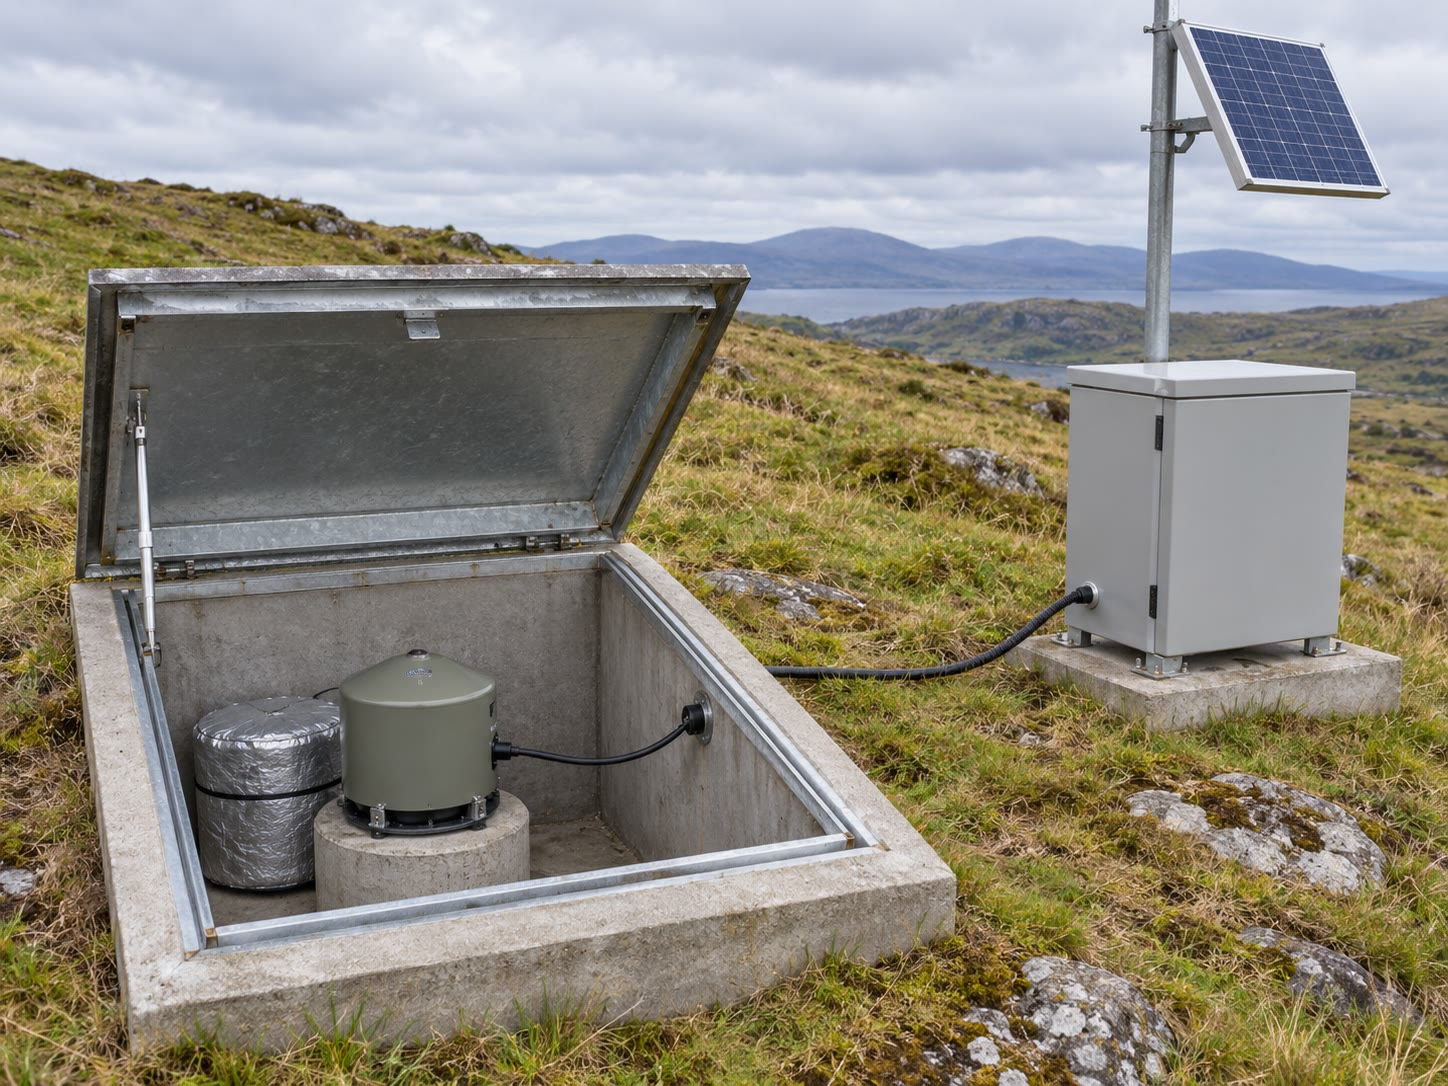
\includegraphics[width=\linewidth]{images/book5/ai/b3-seismic-vault.jpg}

{\scriptsize स्टेशन वॉल्ट में अपने स्तंभ पर एक ब्रॉडबैंड भूकंपमापी
(AI से बनाया गया चित्रण)।}
\end{minipage}
\end{inthefield}

\section{अभ्यास}

\begin{exercise}[$\star$]\label{exo:b3:seismology-imaging:1}
एक P-किरण सतह से निकलती है ($R = \qty{6371}{km}$, $v_0 = \qty{5.80}{km.s^{-1}}$)
\omterm{def:b3:seismology-imaging:ray-parameter}{किरण प्राचल} $p = \qty{500}{s.rad^{-1}}$ के साथ। (क) इसका निर्गम कोण परिकलित कीजिए। (ख) PREM
P-तरंग चाल \qty{771}{km} गहराई पर \qty{11.066}{km.s^{-1}} देता है,
और \qty{871}{km} पर \qty{11.245}{km.s^{-1}} देता है। दोनों गहराइयों पर $r/v$ परिकलित कीजिए और
रैखिक अंतर्वेशन द्वारा किरण की पलटाव गहराई ज्ञात कीजिए।
% ledger: ak135:crust, data:prem
\end{exercise}

\begin{exercise}[$\star$]\label{exo:b3:seismology-imaging:2}
इस अध्याय में PREM से परिकलित P-समय \ang{30} पर \qty{369.6}{s} तथा
\ang{40} पर \qty{455.5}{s} हैं। (क) इनके बीच यात्रा-काल वक्र की प्रवणता का अनुमान लगाइए,
\unit{s} प्रति अंश में और \unit{s.rad^{-1}} में। (ख) इससे पृष्ठ के अनुदिश तरंग-अग्र की
आभासी चाल निकालिए, \unit{km.s^{-1}} में। (ग) \ang{35} पर पहुँचने वाली किरण के
\omterm{def:b3:seismology-imaging:ray-parameter}{पलटाव बिंदु} पर P-चाल क्या है,
यदि वह त्रिज्या \qty{5450}{km} पर पलटती है?
\end{exercise}

\begin{exercise}[$\star$]\label{exo:b3:seismology-imaging:3}
इस अध्याय के लव-तरंग मॉडल में परत के लिए $\beta_1 =
\qty{3.5}{km.s^{-1}}$, $\rho_1 = \qty{2700}{kg.m^{-3}}$ तथा अर्ध-अंतरिक्ष के लिए
$\beta_2 = \qty{4.5}{km.s^{-1}}$, $\rho_2 = \qty{3300}{kg.m^{-3}}$ है।
(क) दोनों कर्तन मापांक परिकलित कीजिए। (ख) \qty{20}{s} पर कला-वेग
\qty{3.79}{km.s^{-1}} है: तरंगदैर्घ्य परिकलित कीजिए और उसकी तुलना परत की
मोटाई \qty{35}{km} से। (ग) \qty{20}{s} पर समूह-वेग \qty{3.384}{km.s^{-1}} और
\qty{100}{s} पर \qty{4.333}{km.s^{-1}} हैं, तो \qty{4000}{km} दूर एक स्टेशन पर
20-s तरंगें 100-s तरंगों के कितने मिनट बाद पहुँचती हैं?
\end{exercise}

\begin{exercise}[$\star$]\label{exo:b3:seismology-imaging:4}
${}_0S_2$ और ${}_0T_2$ के प्रेक्षित आवर्तकाल \qty{53.89}{min} और
\qty{44.01}{min} हैं। (क) इनकी आवृत्तियाँ \unit{mHz} में परिकलित कीजिए। (ख) पृथ्वी
एक दिन में इनमें से प्रत्येक के कितने दोलन पूरे करती है? (ग) दो वर्णक्रमीय शिखर
तभी पृथक किए जा सकते हैं जब अभिलेख कम से कम उनके आवृत्ति-अंतर के व्युत्क्रम
जितनी अवधि तक चले। इन दो विधाओं को पृथक करने के लिए अभिलेख कितनी देर चलना चाहिए?
% ledger: seis5:modes-S, seis5:modes-T
\end{exercise}

\begin{exercise}[$\star\star$]\label{exo:b3:seismology-imaging:5}
त्रिज्या $R$ और एकसमान चाल $v$ वाले गोले में किरणें सीधी जीवाएँ होती हैं।
(क) दिखाइए कि $\Delta$ तक पहुँचने वाली किरण का यात्रा-काल
$T = 2R\sin(\Delta/2)/v$ होता है। (ख) $R = \qty{6371}{km}$ और
$v = \qty{10.0}{km.s^{-1}}$ लेकर \ang{30} और \ang{90} पर $T$ परिकलित कीजिए, और
PREM के समयों \qty{369.6}{s} और \qty{779.7}{s} से तुलना कीजिए। (ग) समझाइए कि एकसमान गोला क्यों
\ang{30} पर क्यों अधिक तेज़ और \ang{90} पर अधिक धीमा है।
\end{exercise}

\begin{exercise}[$\star\star$]\label{exo:b3:seismology-imaging:6}
पॉइसन ठोस पर ($\lambda = \mu$, अतः $\alpha^2 = 3\beta^2$) \omterm{def:b3:seismology-imaging:surface-waves}{रैले तरंग}
की चाल $c$ संतुष्ट करती है, जिसमें $\xi = c^2/\beta^2$ है,
$(2 - \xi)^2 = 4\sqrt{1 - \xi/3}\,\sqrt{1 - \xi}$। (क) इसका वर्ग कीजिए और दिखाइए
कि मूल $(\xi - 4)(3\xi^2 - 12\xi + 8) = 0$ को संतुष्ट करते हैं। (ख) दिखाइए कि
$0 < \xi < 1$ वाला एकमात्र मूल $\xi = 2 - 2/\sqrt3$ है, और $c/\beta$ परिकलित कीजिए।
(ग) ak135 ऊपरी भूपर्पटी में $\beta = \qty{3.46}{km.s^{-1}}$ है। रैले चाल और
\omterm{def:b3:seismology-imaging:surface-waves}{रैले तरंग} का S-तरंग के पीछे विलंब,
\qty{1000}{km} पर परिकलित कीजिए।
% ledger: ak135:crust
\end{exercise}

\begin{exercise}[$\star\star$]\label{exo:b3:seismology-imaging:7}
एक अपवर्तन रेखा के चार स्टेशनों पर हेड-तरंग आगमन, विस्फोट-बिंदु से 50, 100, 150 और
\qty{200}{km} दूरी पर, 9.0, 15.3, 21.5 और \qty{27.9}{s} पर आते हैं, जिनकी त्रुटियाँ
0.1, 0.1, 0.2 और \qty{0.2}{s} हैं। भारित न्यूनतम वर्ग द्वारा $T = a + bx$ का फ़िट कीजिए:
$\mathsf G$ और $\mathsf C_d$ लिखिए, प्रसामान्य समीकरण बनाइए, और
$a$, $b$, उनकी मानक त्रुटियाँ, चाल $1/b$ उसकी त्रुटि के साथ, और
न्यूनतम $\chi^2$ दीजिए। क्या फ़िट स्वीकार्य है?
\end{exercise}

\begin{exercise}[$\star\star$]\label{exo:b3:seismology-imaging:8}
एक किरण दो कोशिकाओं को पार करती है, जिनकी लंबाइयाँ \qty{30}{km} और \qty{40}{km} हैं, और
इसका अवशिष्ट \qty{0.50}{s} है। (क) $\mathsf N = \mathsf G^{\mathsf T}
\mathsf G$ विचित्र क्यों है? (ख) वे मॉडल, जो अवशिष्ट को ठीक-ठीक फ़िट करते हैं, उनमें से
न्यूनतम मानदंड वाला मॉडल $\mathbf m = \mathsf G^{\mathsf T}(\mathsf G\mathsf
G^{\mathsf T})^{-1}\mathbf d$ है: उसे परिकलित कीजिए। (ग) आव्यूह
$\mathsf R = \mathsf G^{\mathsf T}(\mathsf G\mathsf G^{\mathsf T})^{-1}\mathsf G$
और उसका ट्रेस परिकलित कीजिए। (घ) यदि वास्तविक विसंगति केवल पहली
कोशिका में \qty{0.01}{s.km^{-1}} है, तो क्या पुनर्प्राप्त होता है?
\end{exercise}

\begin{exercise}[$\star\star$]\label{exo:b3:seismology-imaging:9}
प्रावार का एक स्लैब-क्षेत्र अपने परिवेश से \qty{3}{\percent} तेज़ है,
जहाँ $v = \qty{9.0}{km.s^{-1}}$ है। (क) इसमें से ऊर्ध्वाधर रूप से गुजरने वाली किरण का
\qty{200}{km} लंबाई में, \cref{prop:b3:seismology-imaging:linear} द्वारा, अवशिष्ट
और ठीक-ठीक परिकलित कीजिए। (ख) उसकी \qty{100}{km} मोटाई को स्लैब के अभिलंब से
\ang{40} पर पार करने वाली किरण के लिए भी यही कीजिए। (ग) रैखिकीकरण की
सापेक्ष त्रुटि क्या है?
\end{exercise}

\begin{exercise}[$\star\star\star$]\label{exo:b3:seismology-imaging:10}
\cref{thm:b3:seismology-imaging:love} में, कोटि $n$ का एक अधिस्वर केवल
पर्याप्त छोटे आवर्तकालों पर विद्यमान है। (क) दिखाइए कि इसके कटऑफ़ पर इसका कला-वेग
$\beta_2$ और $kHq_1 = n\pi$ है। (ख) कटऑफ़ कोणीय आवृत्ति
$\omega_n = n\pi\beta_1\beta_2/\bigl(H\sqrt{\beta_2^2 - \beta_1^2}\bigr)$ निगमित कीजिए।
(ग) अध्याय के मॉडल के लिए प्रथम अधिस्वर का कटऑफ़ आवर्तकाल
($H = \qty{35}{km}$, $\beta_1 = 3.5$, $\beta_2 = \qty{4.5}{km.s^{-1}}$) परिकलित कीजिए।
(घ) दिखाइए कि मूल विधा का कोई कटऑफ़ नहीं है, और उसका कला-वेग
लघु आवर्तकालों पर $\beta_1$ की ओर प्रवृत्त होता है।
\end{exercise}

\begin{exercise}[$\star\star\star$]\label{exo:b3:seismology-imaging:11}
अभ्यास 8 की किरण लीजिए, इकाई आँकड़ा त्रुटि के साथ। (क) दिखाइए कि किसी भी
$\varepsilon > 0$ के लिए, $(\mathsf G^{\mathsf T}\mathsf G + \varepsilon^2\mathsf
I)^{-1}\mathsf G^{\mathsf T} = \mathsf G^{\mathsf T}(\mathsf G\mathsf
G^{\mathsf T} + \varepsilon^2\mathsf I)^{-1}$ सत्य है। (ख) अवमंदित विभेदन
आव्यूह $\mathsf R_\varepsilon = \mathsf G^{\mathsf T}\mathsf G/(\|\mathbf g\|^2 +
\varepsilon^2)$ निगमित कीजिए, जहाँ $\mathbf g = (30, 40)$ है, और उसका ट्रेस। (ग)
$\varepsilon^2 = 0$, 2500 और \num{10000} के लिए ट्रेस और आँकड़ा अवशिष्ट
(\unit{km^2} में) परिकलित कीजिए। समझौते का वर्णन कीजिए।
\end{exercise}

\begin{exercise}[$\star\star\star$]\label{exo:b3:seismology-imaging:12}
अभ्यास 5 के एकसमान गोले में: (क) \cref{thm:b3:seismology-imaging:benndorf} द्वारा
दिखाइए कि $p(\Delta) = (R/v)\cos(\Delta/2)$ है, और इसकी जाँच $p$ की परिभाषा
(जीवा का निर्गम कोण) से कीजिए।
(ख) दिखाइए कि $\Delta_1$ तक पहुँचने वाली किरण $r_1 = R\cos(\Delta_1/2)$ पर पलटती है।
(ग) यह स्वीकार करते हुए कि $\int_0^{\Delta_1}\operatorname{arccosh}\bigl(\cos(\Delta/2)
/\cos(\Delta_1/2)\bigr)\,\mathrm d\Delta = \pi\ln\bigl(1/\cos(\Delta_1/2)\bigr)$,
दिखाइए कि हर्ग्लोट्ज़--वीशर्ट सूत्र $r_1$ और वेग $v$ लौटाता है।
\end{exercise}

\section{समस्या: स्टेशन K के नीचे का स्लैब}

\begin{problem}[{सप्ताहांत समस्या --- किरणें, लव तरंगें और लघु
टोमोग्राफ़ी, एक काल्पनिक स्टेशन के नीचे}]
\label{pb:b3:seismology-imaging:1}
% values: calc/ch01.py (invented station and models; Love-wave model as in the chapter)
स्टेशन K एक महाद्वीप पर एक क्षेपण क्षेत्र के ऊपर स्थित है। यह समस्या इसके अभिलेखों का
तीन प्रकार से उपयोग करती है: किरणें उसकी भूपर्पटी में, उसके पार लव तरंगों का परिक्षेपण,
और नीचे प्रावार की एक लघु टोमोग्राफ़ी।

\medskip
\noindent\textbf{भाग I --- प्रवणता में किरणें।} इतनी छोटी दूरियों पर, जहाँ पृथ्वी की वक्रता की
उपेक्षा की जा सके, K के नीचे P वेग गहराई के साथ रैखिक रूप से बढ़ता है,
$v(z) = v_0 + gz$, जहाँ $v_0 = \qty{5.0}{km.s^{-1}}$ और
$g = \qty{0.05}{s^{-1}}$ ($z$ km में)।
\begin{enumerate}
  \item समतल परतों में स्नेल का नियम $p = \sin i/v$ स्थिर रखता है। एक किरण K से
        $\sin i_0 = 0.8$ के साथ निकलती है: $i_0$ और $p$ परिकलित कीजिए।
  \item यह किस गहराई पर पलटती है, और वहाँ वेग क्या है?
  \item दिखाइए कि किरण के अनुदिश $\mathrm di/\mathrm ds = pg$ है, इसलिए वह
        वृत्त का एक चाप है; उसकी त्रिज्या और उसके केंद्र की गहराई दीजिए।
  \item वह क्षैतिज दूरी $X$ परिकलित कीजिए जिस पर किरण
        पृष्ठ पर लौटती है।
  \item दिखाइए कि $\mathrm dT = \mathrm di/(g\sin i)$ है, और यात्रा-काल
        $T$ ठीक-ठीक परिकलित कीजिए।
  \item $X$ और $T$ का $p = \qty{0.15}{s.km^{-1}}$ के लिए परिकलित कीजिए, और जाँचिए कि
        दो किरणों के बीच $\Delta T/\Delta X$ का मान
        $p$ के दो मानों के बीच आता है।
\end{enumerate}

\noindent\textbf{भाग II --- लव तरंगें और भूपर्पटी।} K के नीचे की भूपर्पटी एक
परत है, जिसका S वेग $\beta_1 = \qty{3.5}{km.s^{-1}}$ और घनत्व
$\rho_1 = \qty{2.7}{g.cm^{-3}}$ है, और वह $\beta_2 =
\qty{4.5}{km.s^{-1}}$, $\rho_2 = \qty{3.3}{g.cm^{-3}}$ वाले प्रावार के ऊपर है; इसकी मोटाई $H$
अज्ञात है। K और एक पड़ोसी स्टेशन के बीच \omterm{def:b3:seismology-imaging:surface-waves}{लव तरंग} का कला-वेग
मापा जाता है: \qty{3.99}{km.s^{-1}} का मान \qty{25}{s} पर, और \qty{4.25}{km.s^{-1}} का मान
\qty{40}{s} पर।
\begin{enumerate}[resume]
  \item $\mu_1$ और $\mu_2$ को \unit{GPa} में परिकलित कीजिए।
  \item \qty{25}{s} पर $k$, $q_1$ और $q_2$ परिकलित कीजिए।
  \item मूल विधा के परिक्षेपण समीकरण को $H$ के लिए हल कीजिए।
  \item \qty{40}{s} पर भी यही कीजिए। क्या दोनों परिणाम सुसंगत हैं?
  \item दोनों आवर्तकालों के बीच समूह वेग का आकलन
        $\Delta\omega/\Delta k$ के रूप में कीजिए, और उसकी तुलना कला-वेगों से कीजिए।
  \item प्रत्येक आवर्तकाल पर तरंगदैर्घ्य परिकलित कीजिए, और समझाइए कि
        दोनों आवर्तकाल भूपर्पटी और सबसे ऊपरी प्रावार को भिन्न अनुपातों में
        क्यों संवेदित करते हैं।
\end{enumerate}

\noindent\textbf{भाग III --- चार कोशिकाओं में एक टोमोग्राफ़ी।} K के नीचे, ऊर्ध्वाधर काट में प्रावार का एक खंड,
\qty{200}{km} गुणा \qty{200}{km} का, चार वर्गाकार कोशिकाओं में विभाजित है,
प्रत्येक \qty{100}{km} की: 1 (ऊपर बाएँ), 2 (ऊपर दाएँ), 3 (नीचे बाएँ)
और 4 (नीचे दाएँ); खाई और महासागर बाईं ओर हैं। संदर्भ वेग $v_0 = \qty{8.0}{km.s^{-1}}$ है।
एक आदर्श प्रयोग में छह सीधी किरणें इसे पार करती हैं: A ऊपरी पंक्ति के साथ (कोशिकाएँ 1
और 2), B निचली पंक्ति के साथ (3 और 4), C बाएँ स्तंभ के नीचे (1 और 3), D
दाएँ स्तंभ के नीचे (2 और 4), E 1 और 4 से होकर विकर्ण के साथ, F 2 और 3 से होकर
विकर्ण के साथ। उनके अवशिष्ट ये हैं:
\begin{center}
\small
\begin{tabular}{lcccccc}
\hline
किरण & A & B & C & D & E & F \\
$\delta t$ (\unit{s}) & $0.16$ & $-0.48$ & $-0.36$ & $0.11$ & $-0.15$ & $-0.27$ \\
त्रुटि $\sigma$ (\unit{s}) & 0.05 & 0.05 & 0.05 & 0.05 & 0.10 & 0.10 \\
\hline
\end{tabular}
\end{center}
मॉडल $\mathbf m$ को कोशिकाओं के मंदता-विचलन मानिए,
\unit{ms.km^{-1}} में ($\qty{1}{ms.km^{-1}} = \qty{e-3}{s.km^{-1}}$), ताकि $\mathsf G$ की प्रविष्टियाँ
\unit{km} में किरण-लंबाइयाँ हों, जिन्हें 1000 से भाग दिया गया है।
\begin{enumerate}[resume]
  \item $\mathsf G$ लिखिए, जो एक $6\times4$ आव्यूह है।
  \item दिखाइए कि $\mathsf N = \mathsf G^{\mathsf T}\mathsf C_d^{-1}\mathsf G$
        की पंक्तियाँ $(10, 4, 4, 2)$, $(4, 10, 2, 4)$, $(4, 2, 10, 4)$ और
        $(2, 4, 4, 10)$ हैं।
  \item $\mathbf b = \mathsf G^{\mathsf T}\mathsf C_d^{-1}\mathbf d$ परिकलित कीजिए।
  \item जाँचिए कि $(1,1,1,1)$, $(1,-1,-1,1)$, $(1,1,-1,-1)$ और $(1,-1,1,-1)$
        $\mathsf N$ के आइगेनसदिश हैं, जिनके आइगेनमान 20, 4, 8 और 8 हैं, और
        निष्कर्ष निकालिए कि $\mathsf N^{-1}$ की पंक्तियाँ $(11, -4, -4, 1)/80$,
        $(-4, 11, 1, -4)/80$, $(-4, 1, 11, -4)/80$ और $(1, -4, -4, 11)/80$ हैं।
  \item \omterm{thm:b3:seismology-imaging:wls}{भारित न्यूनतम-वर्ग अनुमान} $\hat{\mathbf m}$ परिकलित कीजिए।
  \item इसे सापेक्ष वेग विचलन $\delta v/v_0$ प्रतिशत में बदलिए।
  \item प्रत्येक कोशिका की मानक त्रुटि \unit{ms.km^{-1}} में और प्रतिशत में दीजिए,
        और कोशिकाओं 1 और 2 के बीच, तथा कोशिकाओं 1 और 4 के बीच सहसंबंध दीजिए।
        उनके चिह्नों की व्याख्या कीजिए।
  \item फ़िट के बाद छह किरणों के अवशिष्ट और न्यूनतम
        $\chi^2$ परिकलित कीजिए। क्या यह दिए गए त्रुटियों से सुसंगत है?
\end{enumerate}

\noindent\textbf{भाग IV --- अवमंदन, विभेदन और स्लैब।}
\begin{enumerate}[resume]
  \item $\varepsilon^2 = 4$ के लिए ($\mathsf N$ की इकाइयों में) $\mathsf R = (\mathsf N + 4\mathsf I)^{-1}\mathsf N$ के
        आइगेनमान दीजिए, और
        दिखाइए कि $\mathsf R$ का विकर्ण $2/3$ है, कोशिकाओं के बीच प्रविष्टियाँ $1/12$ हैं,
        जो एक पंक्ति या स्तंभ की किरण साझा करती हैं, और कोशिकाओं 1 और 4 के बीच
        तथा 2 और 3 के बीच $0$ है।
  \item कोशिका 3 का अवमंदित अनुमान और उसका वेग विचलन परिकलित कीजिए। वह
        अनवमंदित से छोटा क्यों है?
  \item अवमंदित मॉडल का $\chi^2 = 15.8$ और मानदंड \qty{2.91}{ms.km^{-1}} है;
        अनवमंदित का $\chi^2 = 0.50$ और \qty{4.24}{ms.km^{-1}}; आप किसे रखेंगे,
        और यह समस्या अवमंदन की आवश्यकता क्यों नहीं रखती?
  \item अवमंदित $\mathsf R$ की पंक्ति 3 पढ़िए: कोशिका 3 का अनुमान किन कोशिकाओं के
        साथ धुंधला हो गया है?
  \item कौन-सी कोशिका तेज़ है, और कौन-सी धीमी? तेज़ कोशिका की, जो K के नीचे और
        महासागर की ओर है, क्षेपण क्षेत्र के संदर्भ में व्याख्या कीजिए।
  \item स्लैब कोशिका का P-वेग विचलन प्रतिशत में, उसकी
        मानक त्रुटि के साथ दीजिए।
\end{enumerate}
\end{problem}
